% Chapter Template

\chapter{Ensayos y resultados} % Main chapter title

\label{Chapter4} % Change X to a consecutive number; for referencing this chapter elsewhere, use \ref{ChapterX}


%----------------------------------------------------------------------------------------
%	SECTION 1
%----------------------------------------------------------------------------------------
En este capítulo se detallan los resultados esperados y obtenidos sobre cada una de las pruebas realizadas para validar la integración del sistema y poder comprobar que el alcance funcional logrado es acorde a los esperado.

%\citep{ARTICLE:1}, \citep{BOOK:1}, \citep{BOOK:2}, \citep{WEBSITE:1}.

\section{Banco de pruebas}

Todos los ensayos que se describen en este capítulo fueron efectuados utilizando el diseño físico de red que se muestra en la figura \ref{fig:banco}. Las pruebas funcionales desde dentro de la red local se realizaron con una laptop MacBook Pro y un equipo de escritorio con Windows 10. Para las pruebas de funcionalidad remota se realizaron utilizando un dispositivo móvil Samsung A50 con acceso a la red celular mediante el uso de paquetes de datos a Internet.

\begin{figure}[htbp]
	\centering
	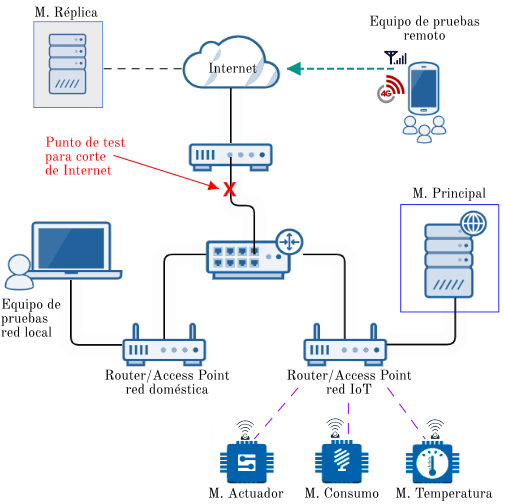
\includegraphics[width=0.82\textwidth]{./Figures/banco2.png}
	\caption{Esquema del banco de pruebas utilizado.}

	\label{fig:banco}
\end{figure}


\section{Pruebas de elección de canal y ancho de banda}
Para las pruebas y análisis de las señales inalámbricas se utilizó el software WiFi Explorer Lite. Es una herramienta de descubrimiento de redes inalámbricas que ayuda a identificar conflictos de canales y problemas de configuración que puedan afectar la conectividad o el rendimiento de la red Wi-Fi de un hogar u oficina \citep{WEBSITE:24}. 

Los fundamentos y consideraciones para la elección del canal y ancho de banda de la señal Wi-Fi que se utilizó, se describieron en el capítulo 3. La elección dependió de las señales circundantes vecinas a la red doméstica donde se instaló el sistema prototipo IoT. La figura \ref{fig:test01} muestra resultado del primer escaneo de las señales y el uso de los canales respectivos así como el solapamiento existente entre ellos. 

De la figura \ref{fig:test01} se describe lo siguiente:

\keyword{Señal WLAN IoT} 
\begin{itemize}
\item SSID: MATRIX-ICF
\item Canal: 10 (configuración automática)
\item Ancho de canal: 40 MHz (configuración automática)
\item Potencia señal: 93\%
\item Seguridad:  WPA2 (PSK)
\item Tasa máxima de transferencia: 300 Mbps
\end{itemize}


\keyword{Señal WLAN doméstica}
\begin{itemize} 
\item SSID: CLARO-B612-D514
\item Canal: 11 (configuración automática)
\item Ancho de canal: 20 MHz (configuración automática)
\item Potencia señal: 64\%
\item Seguridad: WPA2 (PSK)
\item Tasa Máxima de transferencia: 144.4 Mbps
\end{itemize}

El procedimiento de mejora de la configuración de la señal IoT consistió en modificar la configuración por defecto del router/AP al cambiar el canal y reducir el ancho de banda, verificando en cada cambio el comportamiento de las señales en el ambiente y la reducción de solapamiento de los mismos.

La figura \ref{fig:test02} muestra el ancho de banda que ocupa el canal de comunicación de la señal del router sin configurar. Esta configuración por defecto demuestra no ser la más adecuada para el ambiente IoT, debido a que produce interferencias a las señales circundantes.

La figura \ref{fig:test03} muestra las características de la señal inalámbrica doméstica del lugar donde se implementó el sistema IoT prototipo.


%%%%%%%%%%%%%%%%%%%%%%%%%%%%%%%%%%%%%%%%%%%%%%%%%%%
\begin{landscape} % esto es para rotar la pagina e imagen
\begin{figure}[htpb]
\centering 
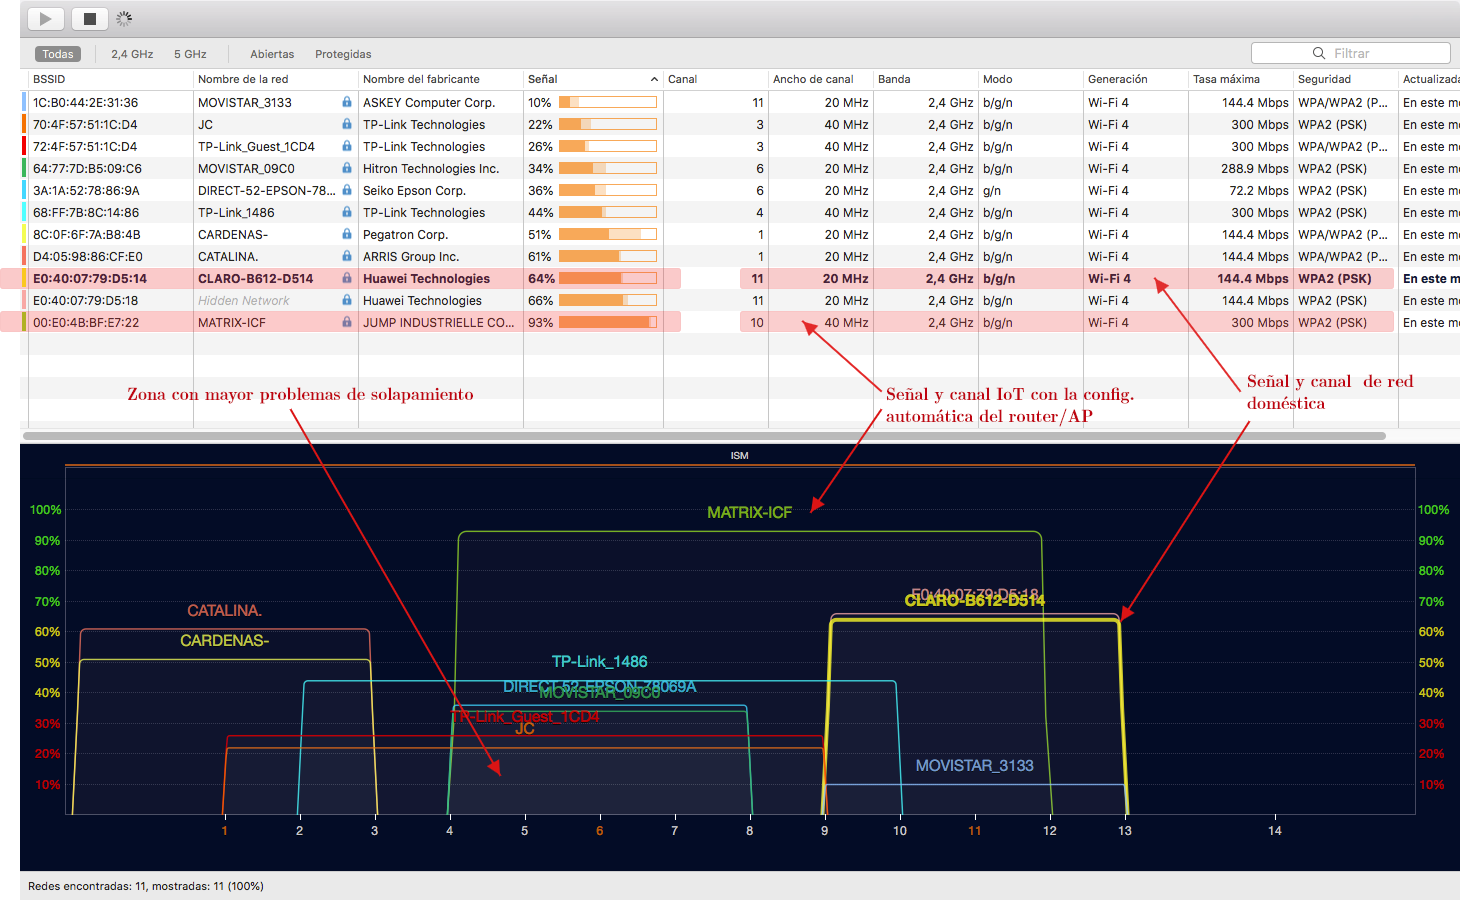
\includegraphics[width=1.5\textwidth]{./Figures/wifi/01.png}
\caption{Estado inicial de las señales Wi-Fi local y circundantes en el ambiente donde se implanto el sistema IoT.}
\label{fig:test01}
\end{figure}
\end{landscape} %

%%%%%%%%%%%%%%%%%%%%%%%%%%%%%%%%%%%%%%%%%%%%%%%%%%%

\begin{landscape} % esto es para rotar la pagina e imagen
\begin{figure}[htpb]
\centering 
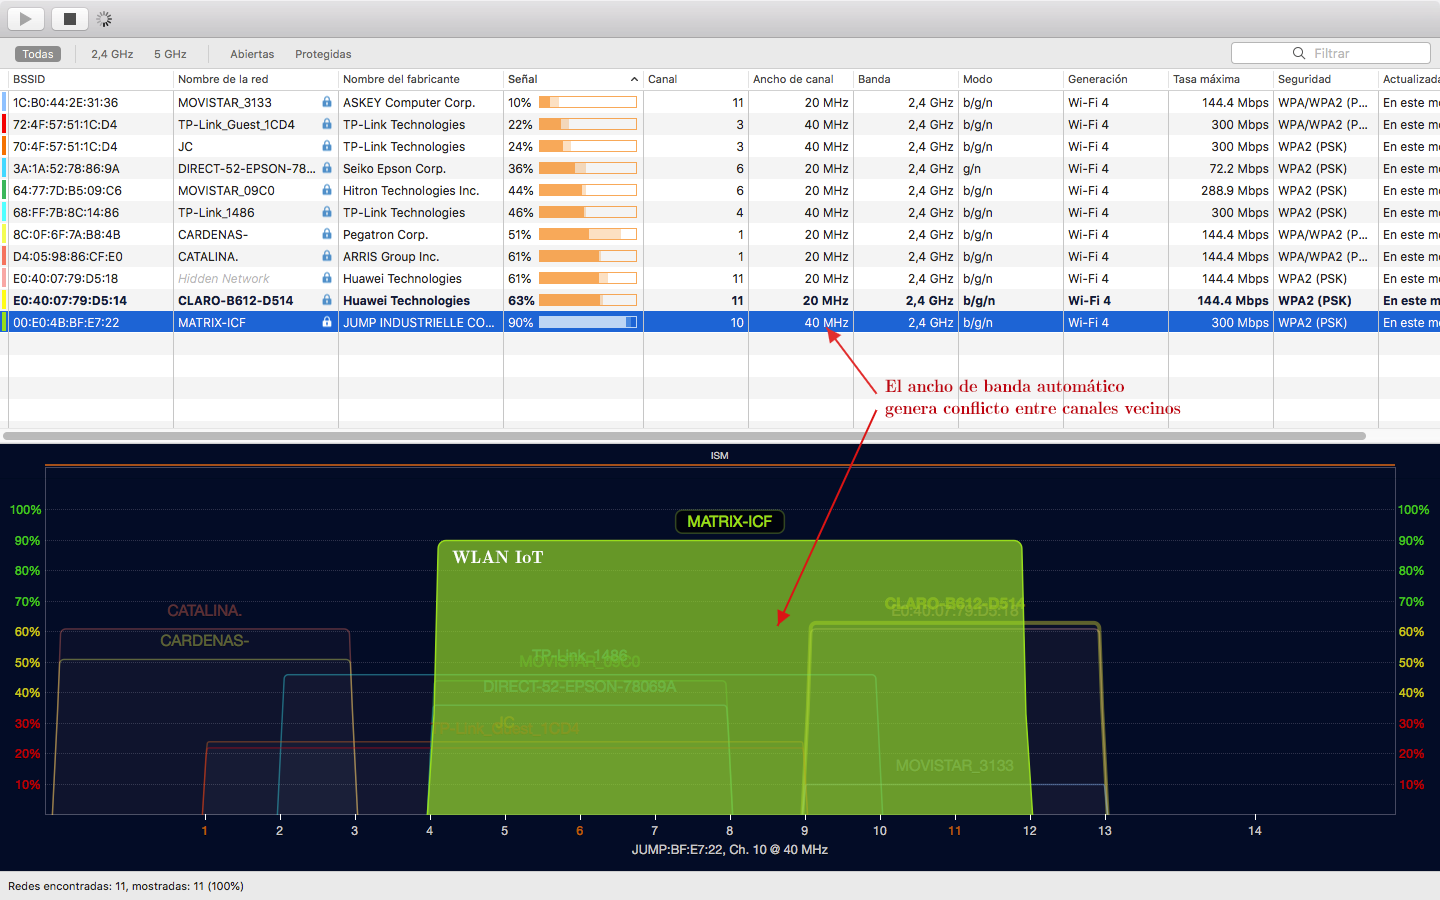
\includegraphics[width=1.5\textwidth]{./Figures/wifi/02.png}
\caption{Ancho de banda de la señal del router para la red IoT con la configuración por defecto del dispositivo.}
\label{fig:test02}
\end{figure}
\end{landscape} %


%%%%%%%%%%%%%%%%%%%%%%%%%%%%%%%%%%%%%%%%%%%%%%%%%%%
\begin{landscape} % esto es para rotar la pagina e imagen
\begin{figure}[htpb]
\centering 
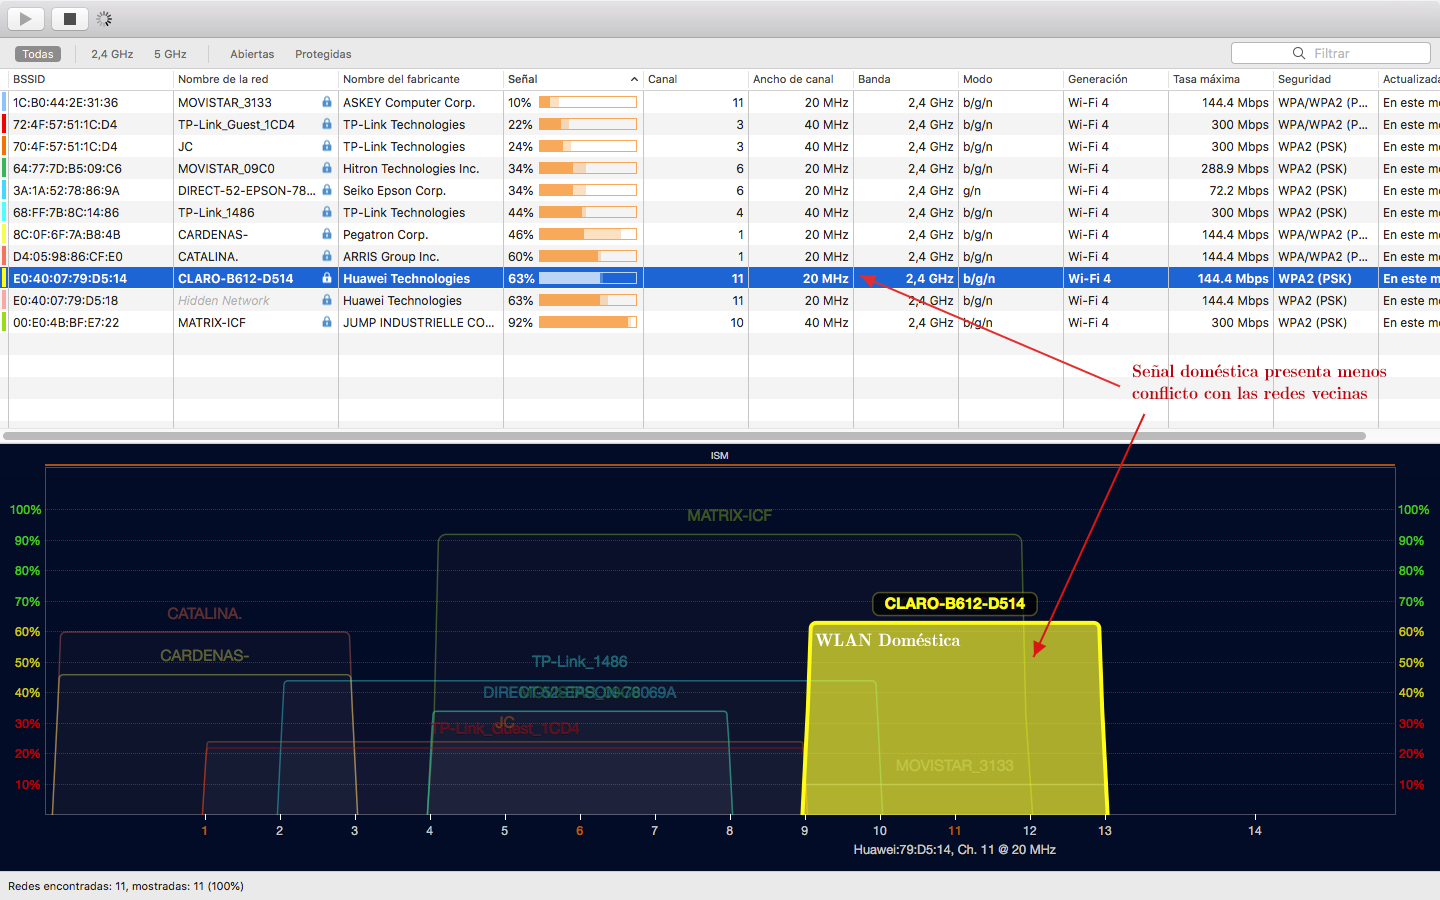
\includegraphics[width=1.5\textwidth]{./Figures/wifi/03.png}
\caption{Ancho de banda  y canal de la señal Wi-Fi doméstica.}
\label{fig:test03}
\end{figure}
\end{landscape} %

%%%%%%%%%%%%%%%%%%%%%%%%%%%%%%%%%%%%%%%%%%%%%%%%%%%%%%%%%%%%%%
El objetivo de usar un software de exploración Wi-Fi es detectar las zonas y canales con mayor interferencia y elegir un canal que tenga la mínima o ninguna intersección con la zona critica. El \emph{software} detectó la zona con mayor solapamiento y lo marcó en color rojo, como se muestra en la figura \ref{fig:test04}, asociado al SSID y al canal que lo causa.

El análisis de las imágenes de señales que genera el \emph{software} de exploración permite conocer cuales podrían ser los canales ideales. El resultado del cambio de canal para la señal destinada a la comunicación IoT, se muestra en la figura \ref{fig:test05}. 

Si se compara la figura \ref{fig:test02} (antes) con la figura \ref{fig:test05} (después), se puede observar la diferencia del canal configurado al mostrar la reducción de interferencias con las señales circundantes.

Al cambiar el canal de la señal IoT, el \emph{software} cambia el color de la zona crítica (de rojo a naranja) en señal que el solapamiento se redujo, demostrando que existe una mejora en la señal de comunicación a utilizar. La figura \ref{fig:test06} muestra el resultado de mejora obtenido.

Las pruebas y cambios de canal para el router/AP se deben realizar durante la instalación y puesta en marcha al sistema IoT y podrán ser actualizados de acuerdo al cronograma establecido para su mantenimiento. 


%%%%%%%%%%%%%%%%%%%%%%%%%%%%%%%%%%%%%%%%%%%%%%%%%%%

\begin{landscape} % esto es para rotar la pagina e imagen
\begin{figure}[htpb]
\centering 
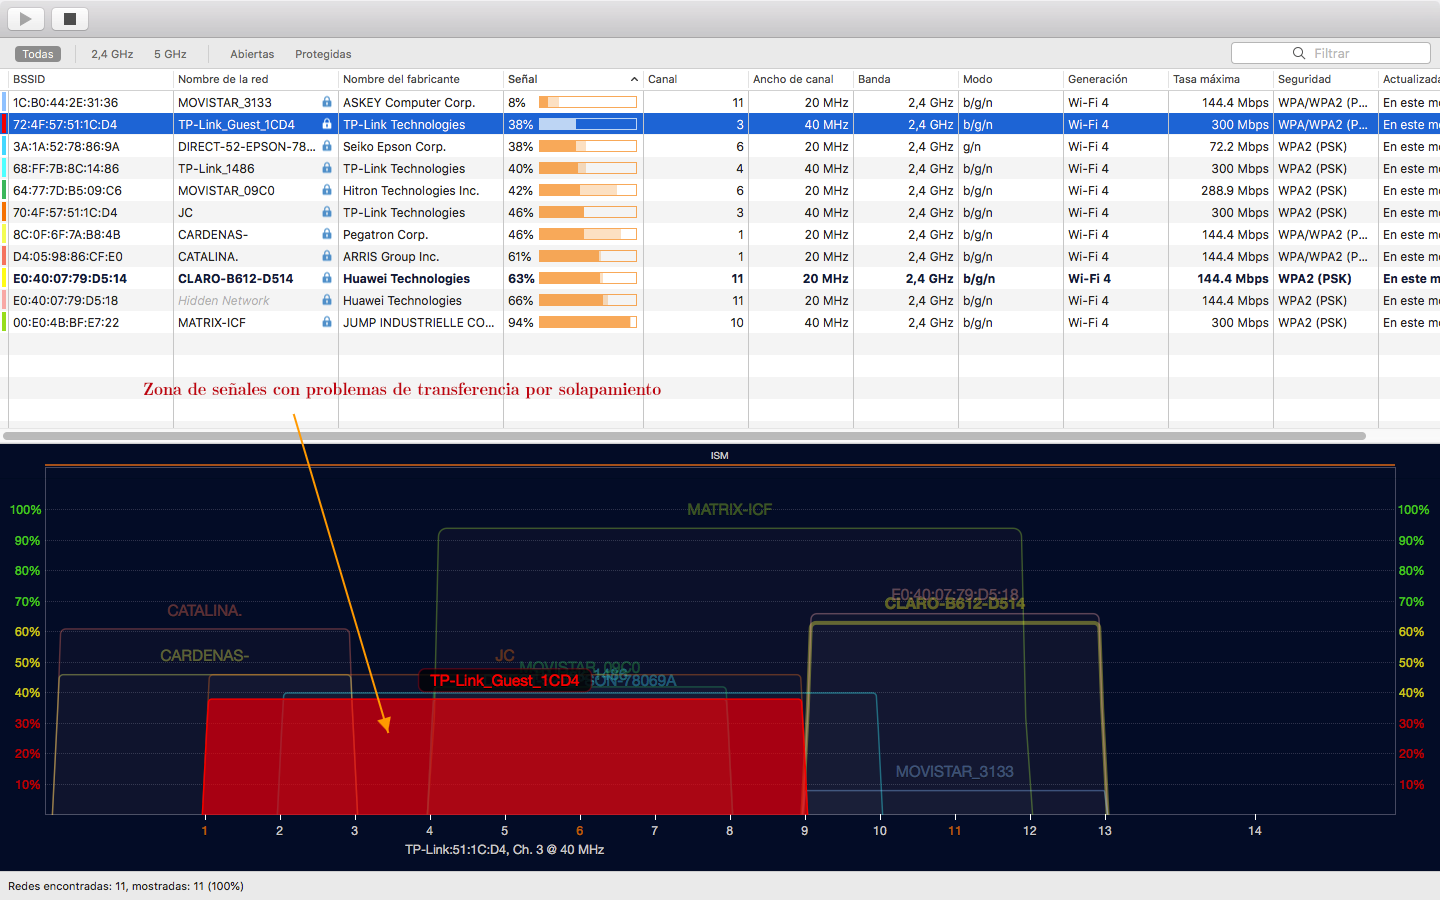
\includegraphics[width=1.5\textwidth]{./Figures/wifi/04.png}
\caption{Zona crítica con mayor interferencia entre los canales de las redes inalámbricas.}
\label{fig:test04}
\end{figure}
\end{landscape} %


%%%%%%%%%%%%%%%%%%%%%%%%%%%%%%%%%%%%%%%%%%%%%%%%%%%

\begin{landscape} % esto es para rotar la pagina e imagen
\begin{figure}[htpb]
\centering 
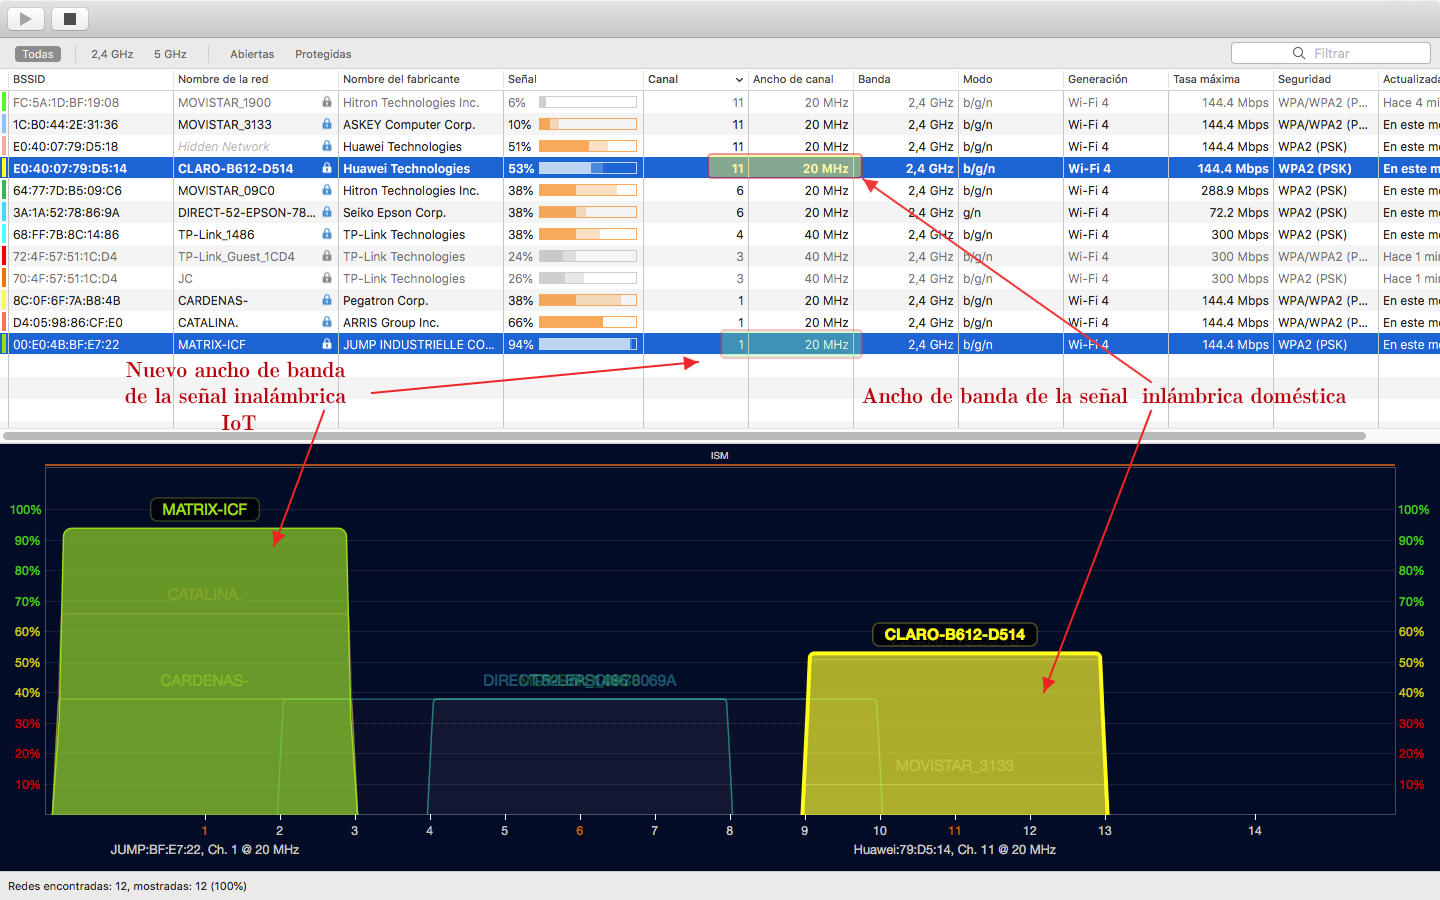
\includegraphics[width=1.5\textwidth]{./Figures/wifi/05.png}
\caption{Ancho de banda y nuevo canal de funcionamiento para las señales IoT y doméstica.}
\label{fig:test05}
\end{figure}
\end{landscape} %


%%%%%%%%%%%%%%%%%%%%%%%%%%%%%%%%%%%%%%%%%%%%%%%%%%%

\begin{landscape} % esto es para rotar la pagina e imagen
\begin{figure}[htpb]
\centering 
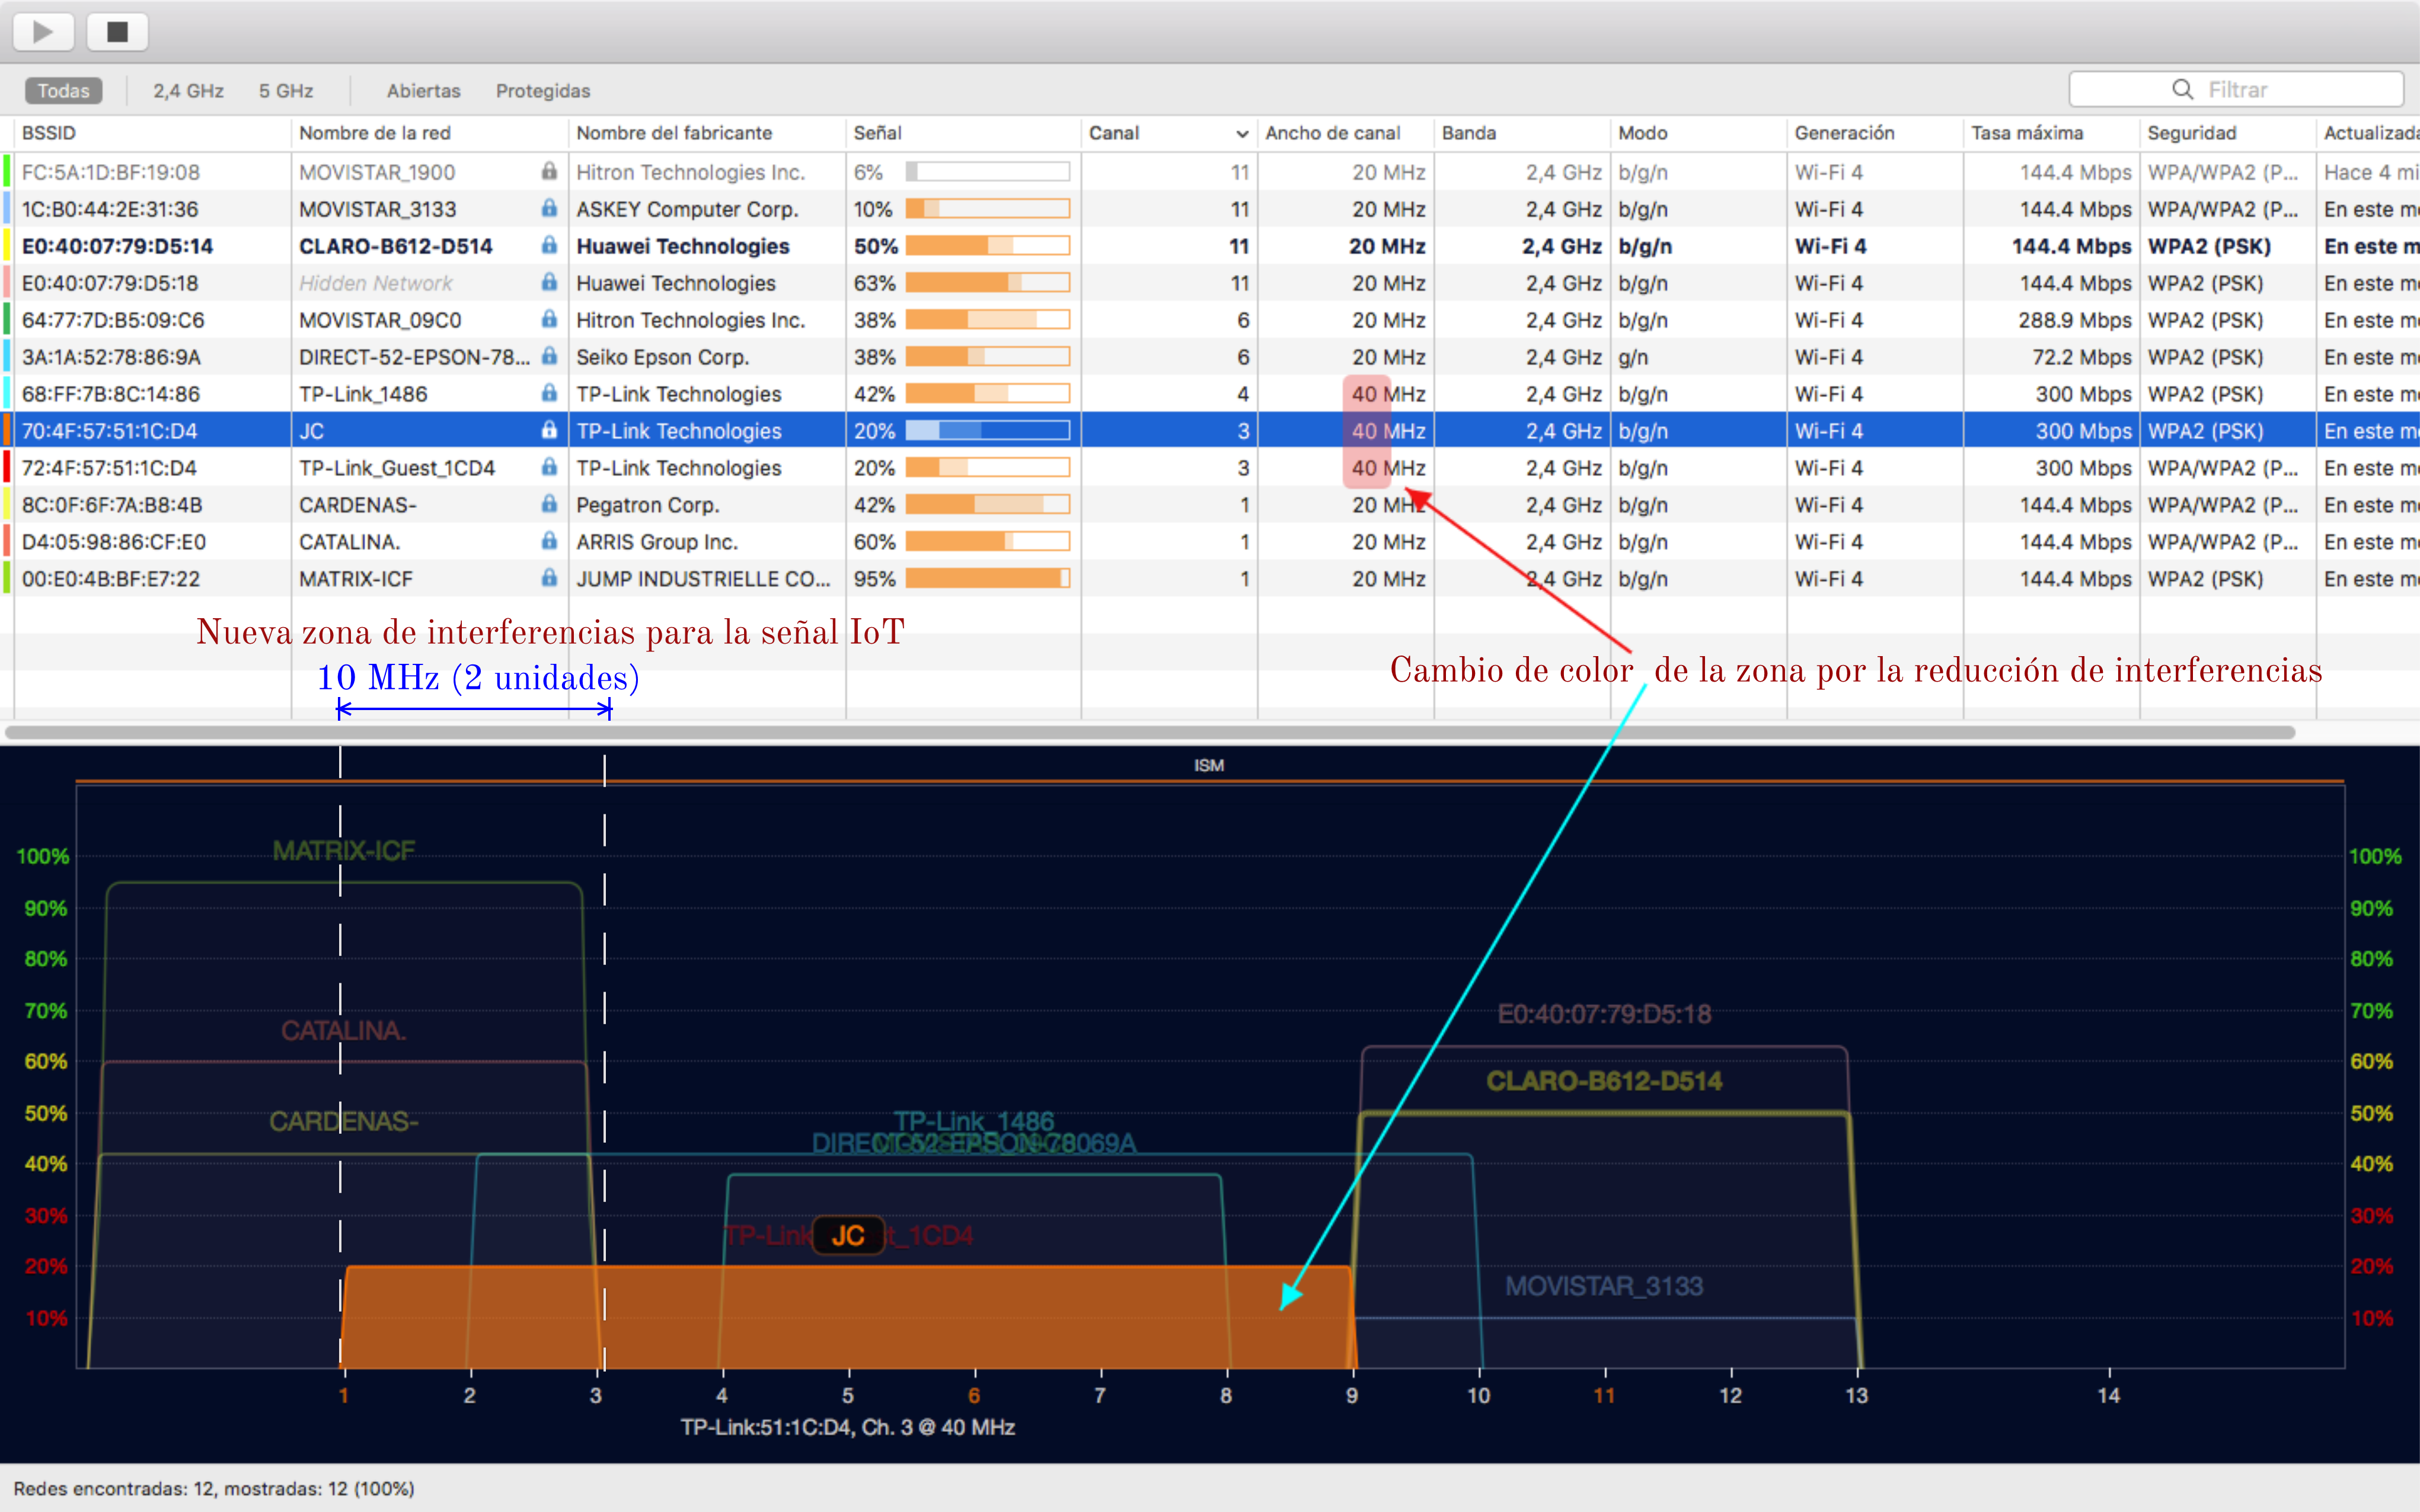
\includegraphics[width=1.5\textwidth]{./Figures/wifi/06.png}
\caption{Zona con reducción de solapamiento después de la configuración manual del router.}
\label{fig:test06}
\end{figure}
\end{landscape} %


\section{Pruebas del módulo de temperatura}

El módulo permite leer las variables físicas de temperatura y humedad del ambiente donde se instaló. La temperatura se muestra en la pantalla OLED del módulo y mas a detalle en el \emph{software} web de monitoreo y control.

La figura \ref{fig:test-temp} muestra la instalación para las pruebas y el valor obtenido en la pantalla OLED. La figura \ref{fig:temp-lectura} muestra los valores obtenidos en el \emph{software} de monitoreo y sus detalles se muestra en la figura \ref{fig:temp-detalle}.

\begin{figure}[htpb]
\centering 
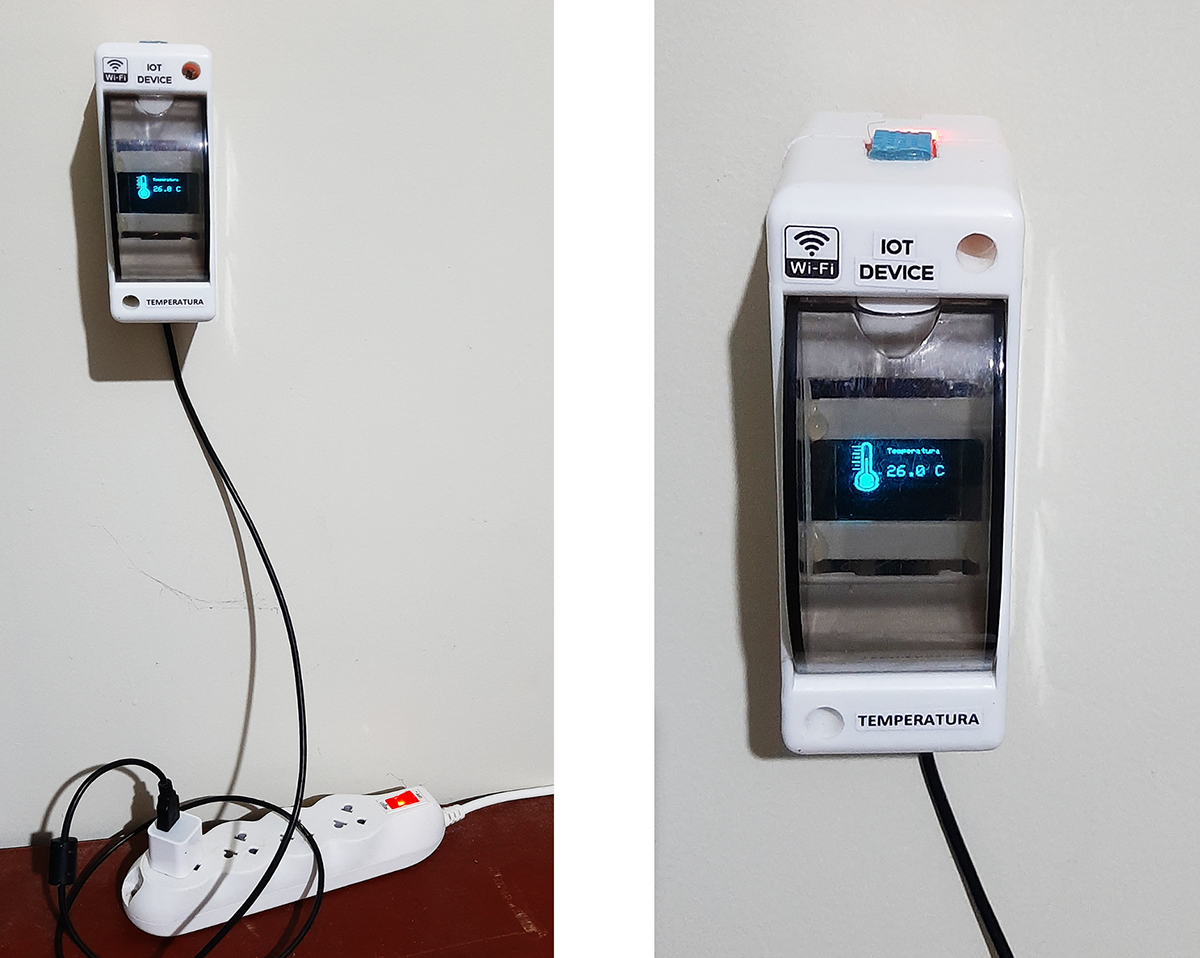
\includegraphics[width=0.9\textwidth]{./Figures/test/temp/test-temp.png}
\caption{Funcionamiento del módulo de temperatura.}
\label{fig:test-temp}
\end{figure}

La figura \ref{fig:test-panel} muestra las características del panel de visualización del módulo en el software.

\begin{figure}[htpb]
\centering 
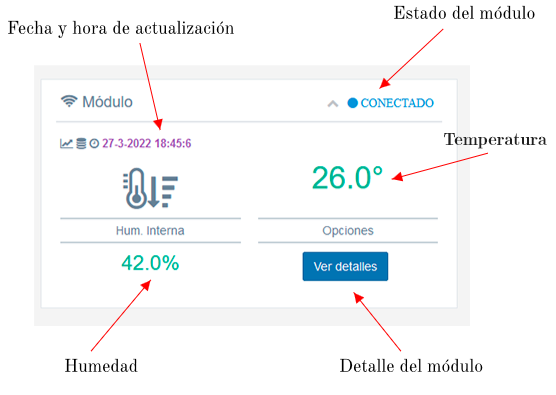
\includegraphics[width=0.65\textwidth]{./Figures/test/temp/panel.png}
\caption{Características del panel de visualización.}
\label{fig:test-panel}
\end{figure}

%%%%%%%%%%%%%%%%%%%%%%%%%%%%%%%%%%%%%%%%%%%%%%%%%%%

\begin{landscape} % esto es para rotar la pagina e imagen
\begin{figure}[htpb]
\centering 
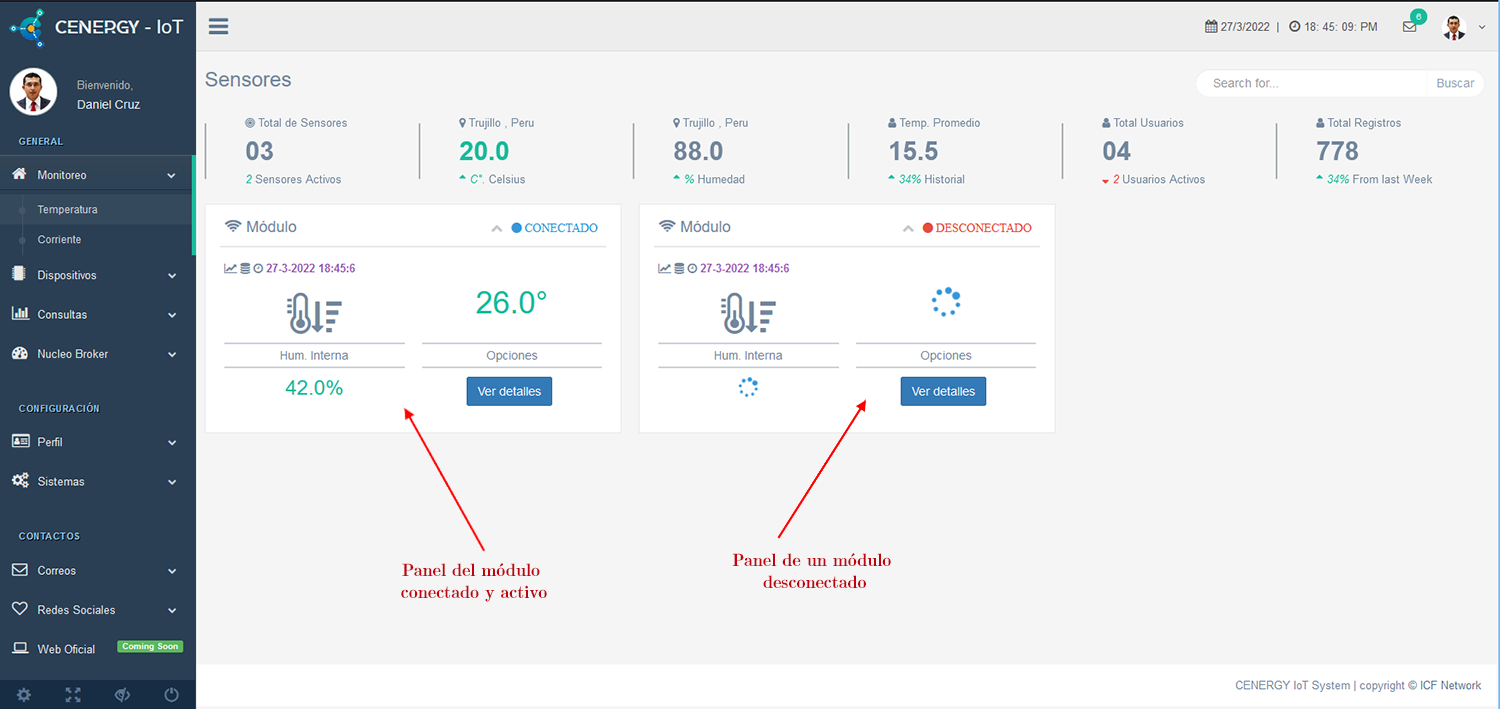
\includegraphics[width=1.7\textwidth]{./Figures/test/temp/lectura.png}
\caption{Monitoreo de los módulos la temperatura en el software.}
\label{fig:temp-lectura}
\end{figure}
\end{landscape} %
%%%%%%%%%%%%%%%%%%%%%%%%%%%%%%%%%%%%%%%%%%%%%%%%%%%


\begin{landscape} % esto es para rotar la pagina e imagen
\begin{figure}[htpb]
\centering 
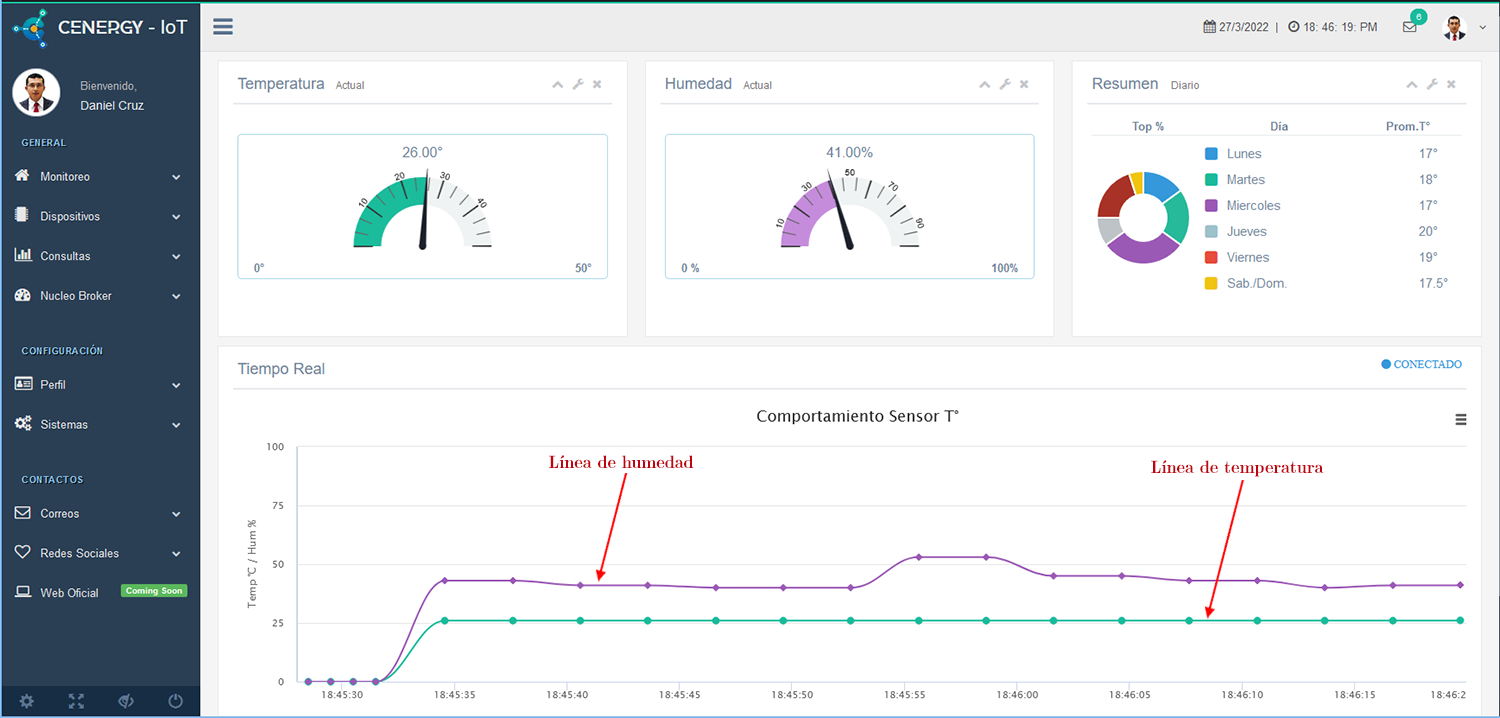
\includegraphics[width=1.7\textwidth]{./Figures/test/temp/detalle.png}
\caption{Detalle del módulo de temperatura conectado y activo.}
\label{fig:temp-detalle}
\end{figure}
\end{landscape} %
%%%%%%%%%%%%%%%%%%%%%%%%%%%%%%%%%%%%%%%%%%%%%%%%%%%

\section{Pruebas del módulo actuador}
Para las pruebas se usó un esquema de conexión como se muestra en la figura \ref{fig:test-esquema}, usando un ventilador como electrodoméstico de consumo. 
\vspace{0.5cm}
\begin{figure}[htpb]
\centering 
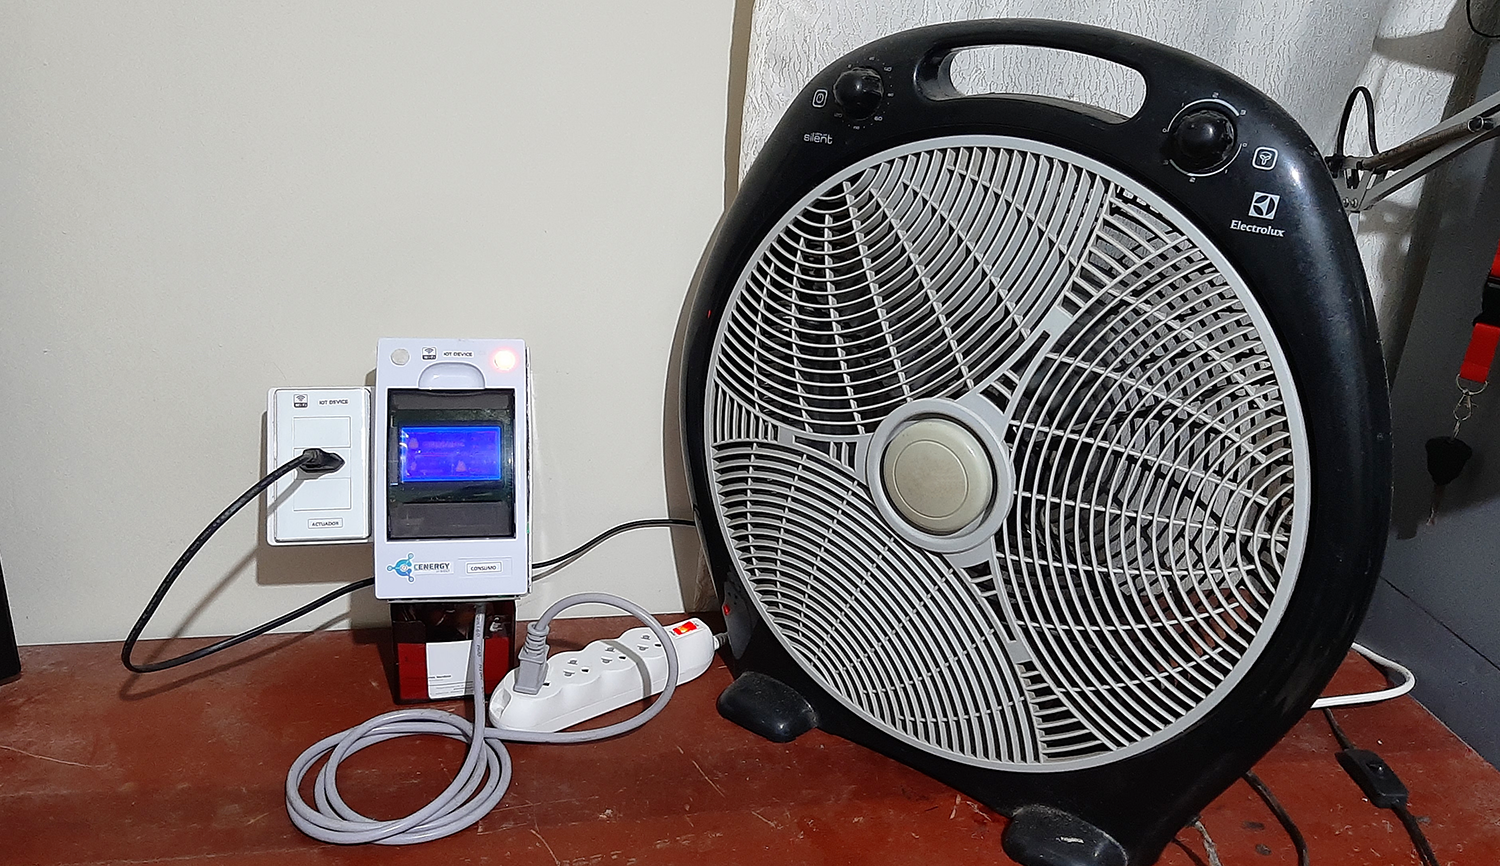
\includegraphics[width=0.87\textwidth]{./Figures/test/consumo/esquema.png}
\caption{Esquema de conexión para pruebas del módulo actuador.}
\label{fig:test-esquema}
\end{figure}

Al implementar el módulo y realizar las pruebas respectivas se demostró que el sensor AC-ZMPT101B es muy sensible en la captura del valor de la tensión. El valor obtenido se contrastó con un multímetro digital dando una diferencia aproximada de +2 V / -2 V. La figura \ref{fig:test-tension} muestra la comprobación de la tensión.

\begin{figure}[htpb]
\centering 
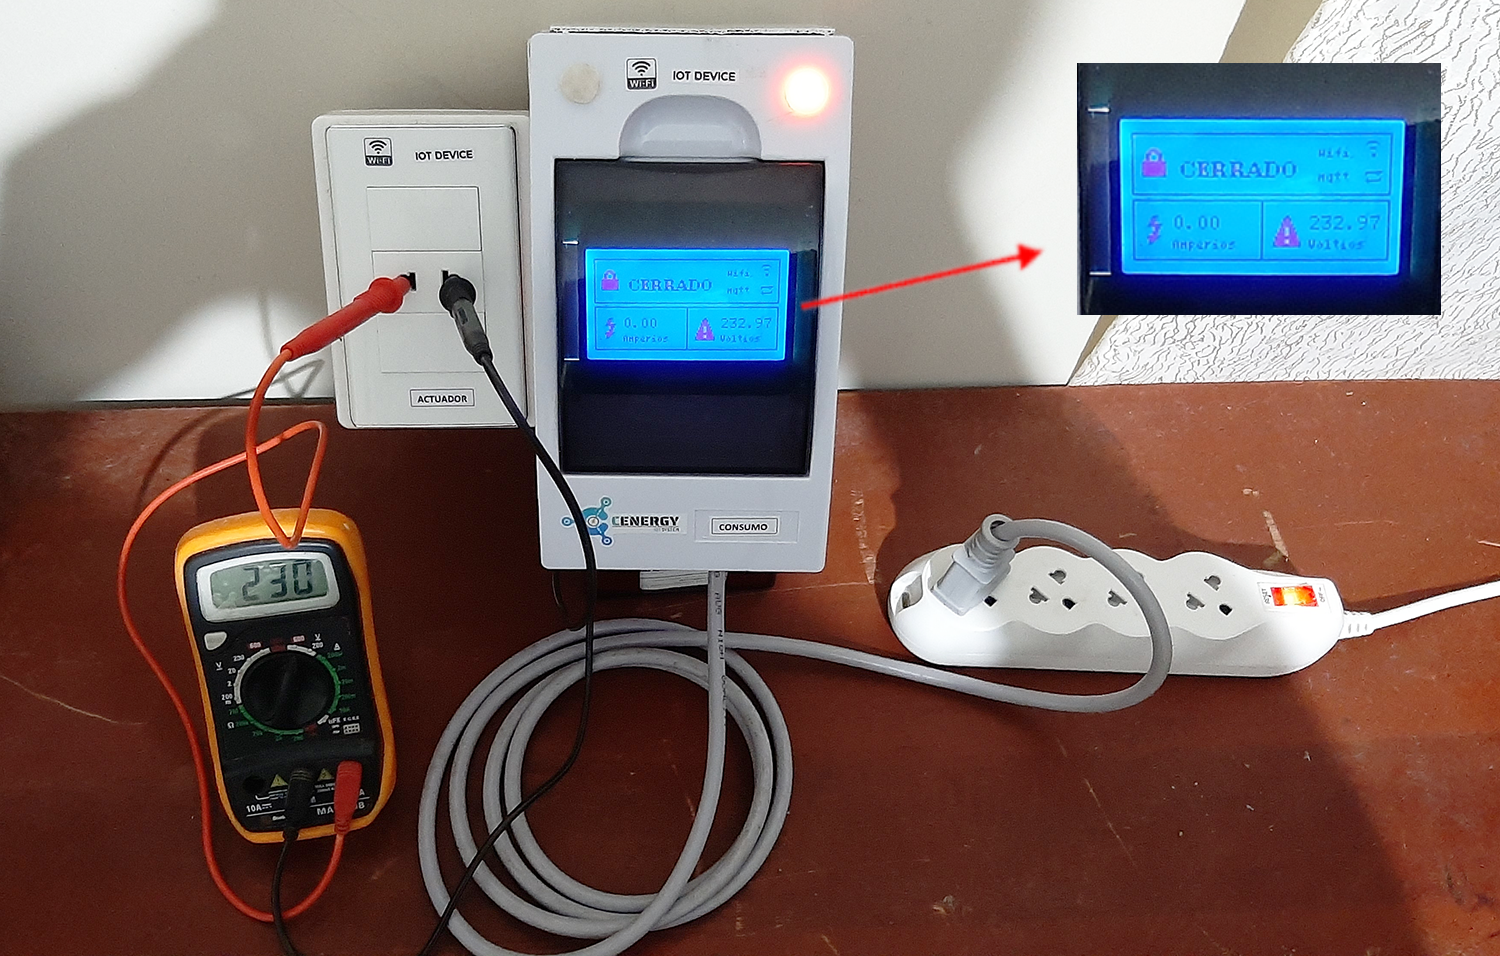
\includegraphics[width=1.0\textwidth]{./Figures/test/consumo/tension2.png}
\caption{Comparación de la medida de la tensión entre el módulo y el multímetro.}
\label{fig:test-tension}
\end{figure}

El módulo permite leer las variables físicas de tensión e intensidad así como el estado del relé actuador. Las lecturas se muestran en su pantalla gráfica como se muestra en la figura \ref{fig:test-activa1} y en la figura \ref{fig:test-activa2}.
\vspace{0.5cm}
\begin{figure}[htpb]
\centering 
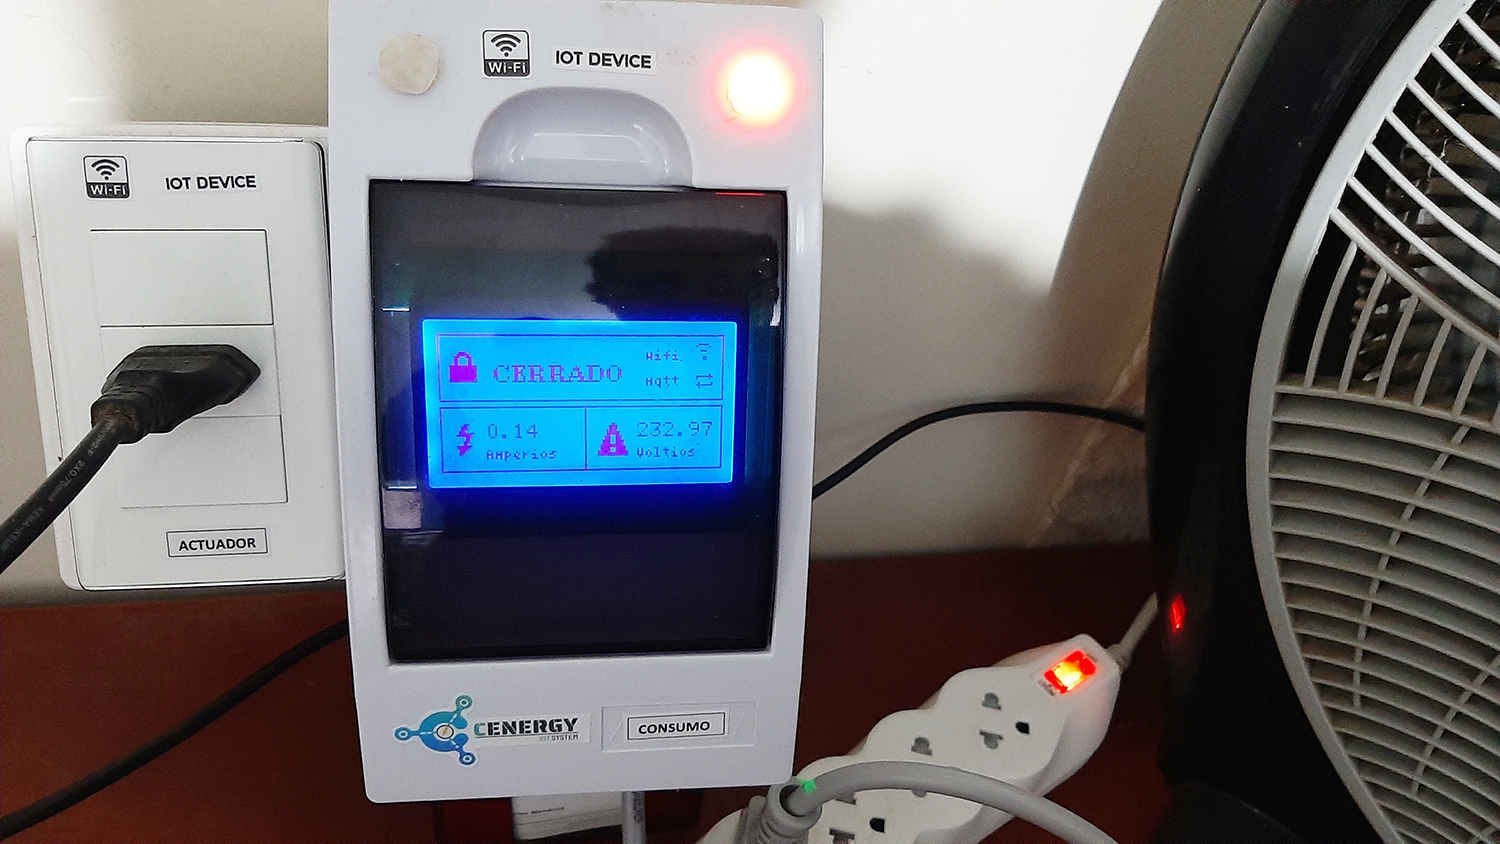
\includegraphics[width=1.0\textwidth]{./Figures/test/consumo/paso.png}
\caption{Módulo con paso de la corriente eléctrica (led rojo indica riesgo eléctrico en la toma de corriente ).}
\label{fig:test-activa1}
\end{figure}

\vspace{0.5cm}
\begin{figure}[htpb]
\centering 
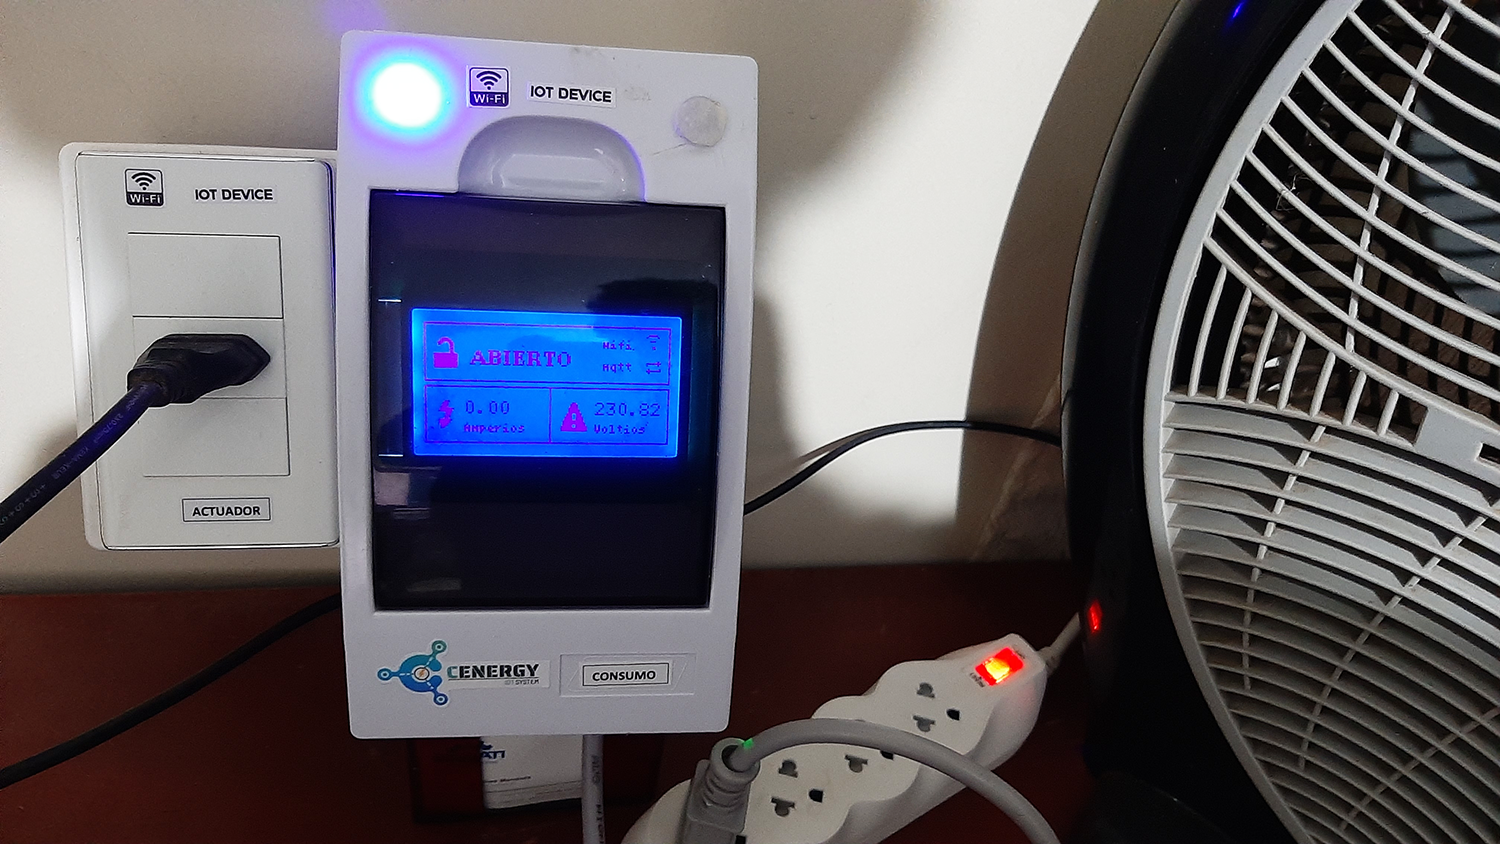
\includegraphics[width=1.0\textwidth]{./Figures/test/consumo/bloqueo.png}
\caption{Módulo con bloqueo de la corriente eléctrica (led azul indica sin riesgo eléctrico en la toma de corriente).}
\label{fig:test-activa2}
\end{figure}

\vspace{0.5cm}
\section{Pruebas de consumo de energía eléctrica}

El consumo que se ha medido en estas pruebas se realizó a un ventilador de casa (modelo antiguo), cuyas características principales son:

\begin{itemize}
\item Marca: ELECTROLUX
\item Tipo:	circuladores de aire con temporizador
\item Modelo: BFV10
\item Número de velocidades: 3
\item Potencia: 30 W
\end{itemize}

La figura \ref{fig:ventilador}  muestra las especificaciones técnicas adheridas en su parte posterior del ventilador. En la actualidad este modelo aún se comercializa pero con un incremento en el número de velocidades y en la potencia de consumo. 

\begin{figure}[htpb]
\centering 
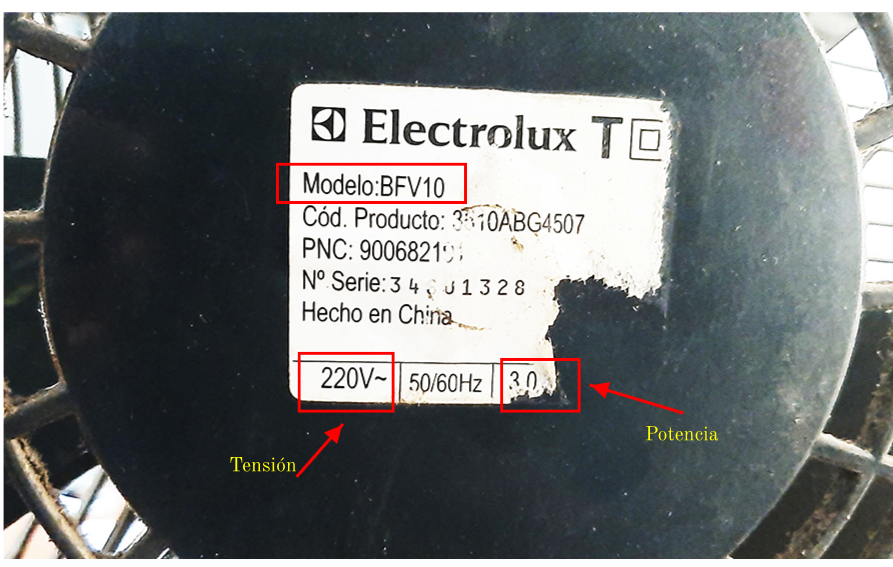
\includegraphics[width=0.7\textwidth]{./Figures/test/consumo/ventilador.png}
\caption{Etiqueta con información técnica del ventilador.}
\label{fig:ventilador}
\end{figure}

Según la guía del organismo supervisor de la inversión en energía (OSINERG - Perú) \citep{BOOK:3}, para calcular el consumo eléctrico, el valor de la potencia  debe ser convertida a Kilowatts (kW), para ello se divide la potencia entre 1000. Para el ventilador usado en la pruebas el valor ideal sería la ecuación \ref{eq:potenciatest2}.

\begin{equation}
	\label{eq:potenciatest2}
	PE = \left( 0.03 \right) kW
\end{equation}

Para comparar el valor obtenido en la formula \ref{eq:potenciatest2}, el módulo de consumo nos permite obtener un valor real de la potencia del ventilador mediante la formula \ref{eq:potenciaform}, las variables de tensión e intensidad de corriente son multiplicadas y se obtiene un valor de potencia en un instante de tiempo. La figura \ref{fig:registroPotencia} muestra las lecturas almacenadas en la base de datos del sistema IoT y en la tabla \ref{tab:tablapotencias} se muestra la comparación del valor ideal con el valor real obtenido desde el módulo de consumo.

\begin{figure}[htpb]
\centering 
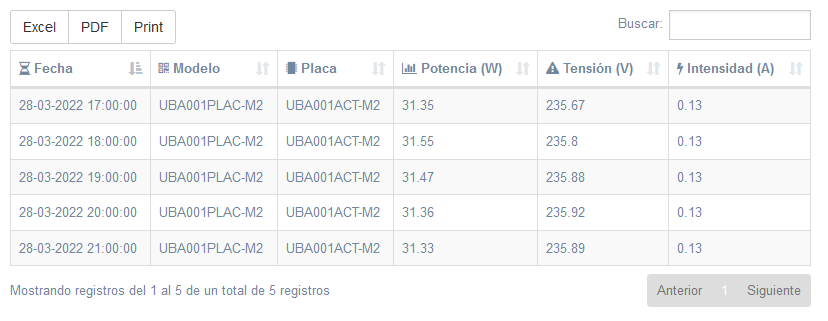
\includegraphics[width=0.95\textwidth]{./Figures/test/consumo/lecturas.png}
\caption{Lecturas de potencia almacenadas en la base de datos del sistema IoT.}
\label{fig:registroPotencia}
\end{figure}

%\vspace{1.0cm}

\begin{table}[h]
	\centering
	\caption[Comparativa de registros de potencias obtenidas]{Comparativa de registros de potencias obtenidas.}
	\begin{tabular}{l c c c}    
		\toprule
		\textbf{P. ideal (W)} 	 & \textbf{P. ideal (kW)}  & \textbf{P. real - módulo (W)} &\textbf{P. real módulo (kW)} \\
		\midrule
		30 & 0.03 & 31.35 & 0.03135\\		
		30& 0.03 & 31.55  &0.03155 \\
		30& 0.03 & 31.47 & 0.03147\\		
		30& 0.03 & 31.36 & 0.03136\\		
		30& 0.03 & 31.33 & 0.03133\\
		\bottomrule
		\hline
	\end{tabular}
	\label{tab:tablapotencias}
\end{table}

El valor de las variables físicas de tensión e intensidad que son necesarias para calcular la  potencia del ventilador, se muestran en el software de monitoreo y control dentro de un conjunto de paneles según la cantidad de módulos registrados en el sistema IoT.

Para facilitar la comprensión de la interfaz gráfica del software, la figura \ref{fig:test-panel5} muestra las características del panel de visualización del módulo en el \emph{software} cuando el actuador permite el paso de la corriente eléctrica. La figura \ref{fig:test-panel4} muestra las características del panel de visualización del módulo en el \emph{software} cuando el actuador bloquea el paso de la corriente eléctrica .

\begin{figure}[htpb]
\centering 
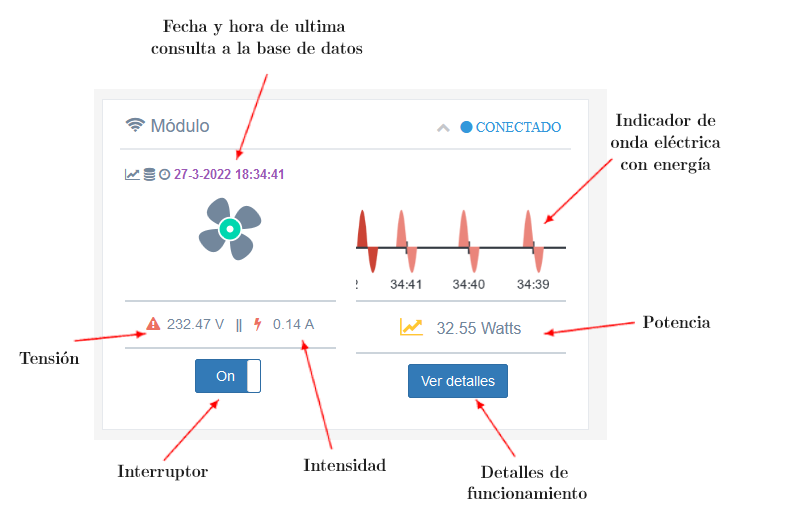
\includegraphics[width=1.0\textwidth]{./Figures/test/consumo/panel5.png}
\caption{Panel de visualización del módulo con paso de corriente eléctrica.}
\label{fig:test-panel5}
\end{figure}

%\vspace{0.5cm}

\begin{figure}[htpb]
\centering 
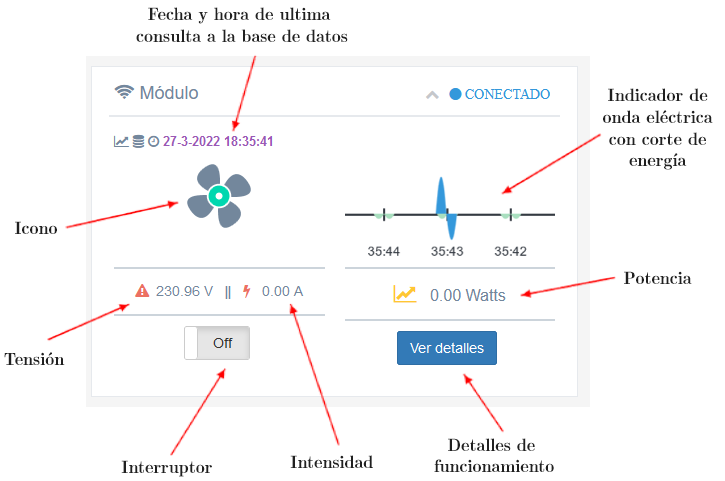
\includegraphics[width=1.0\textwidth]{./Figures/test/consumo/panel4.png}
\caption{Panel de visualización del módulo con bloqueo de la corriente eléctrica.}
\label{fig:test-panel4}
\end{figure}

Las variables de tensión, intensidad y potencia eléctrica del electrodoméstico conectado a él, se pueden visualizar en el \emph{software} de monitoreo y control así como los detalles de su funcionamiento en tiempo real. La figura \ref{fig:dashboard-v1} y \ref{fig:dashboard-v2} ilustran lo mencionado.

Para calcular el monto a pagar por el usuario se consideraron consumos facturados y consumos no facturados. Los consumos facturados son aquellos registros resumen de un conjunto de registros temporales que se dieron dentro de un intervalo de tiempo. Por ejemplo, dentro del intervalo '28-03-2022 16:00:00' y '28-03-2022 17:00:00' se capturan aproximadamente 1800 lecturas de potencia, para considerar la facturación se obtiene la media aritmética del valor de potencia del conjunto y se almacena como único registro en la tabla de facturación con fecha y hora '28-03-2022 17:00:00', posteriormente se procede a eliminar los 1800 registros temporales. Los consumos no facturados son los registros temporales. 

Se realizó un muestreo de 5 horas de funcionamiento continuo del ventilador y se obtuvieron los resultados que se muestran en la figura \ref{fig:dashboard-consumo}. El \emph{dashboard} del \emph{software} de monitoreo y control ofrece una vista resumida del subtotal y total a pagar así como un gráfico interactivo de potencia vs costo de consumo por hora.

%%%%%%%%%%%%%%%%%%%%%%%%%%%%%%%%%%%%%%%%%%%%%%%%%%%
\begin{landscape} % esto es para rotar la pagina e imagen
\begin{figure}[htpb]
\centering 
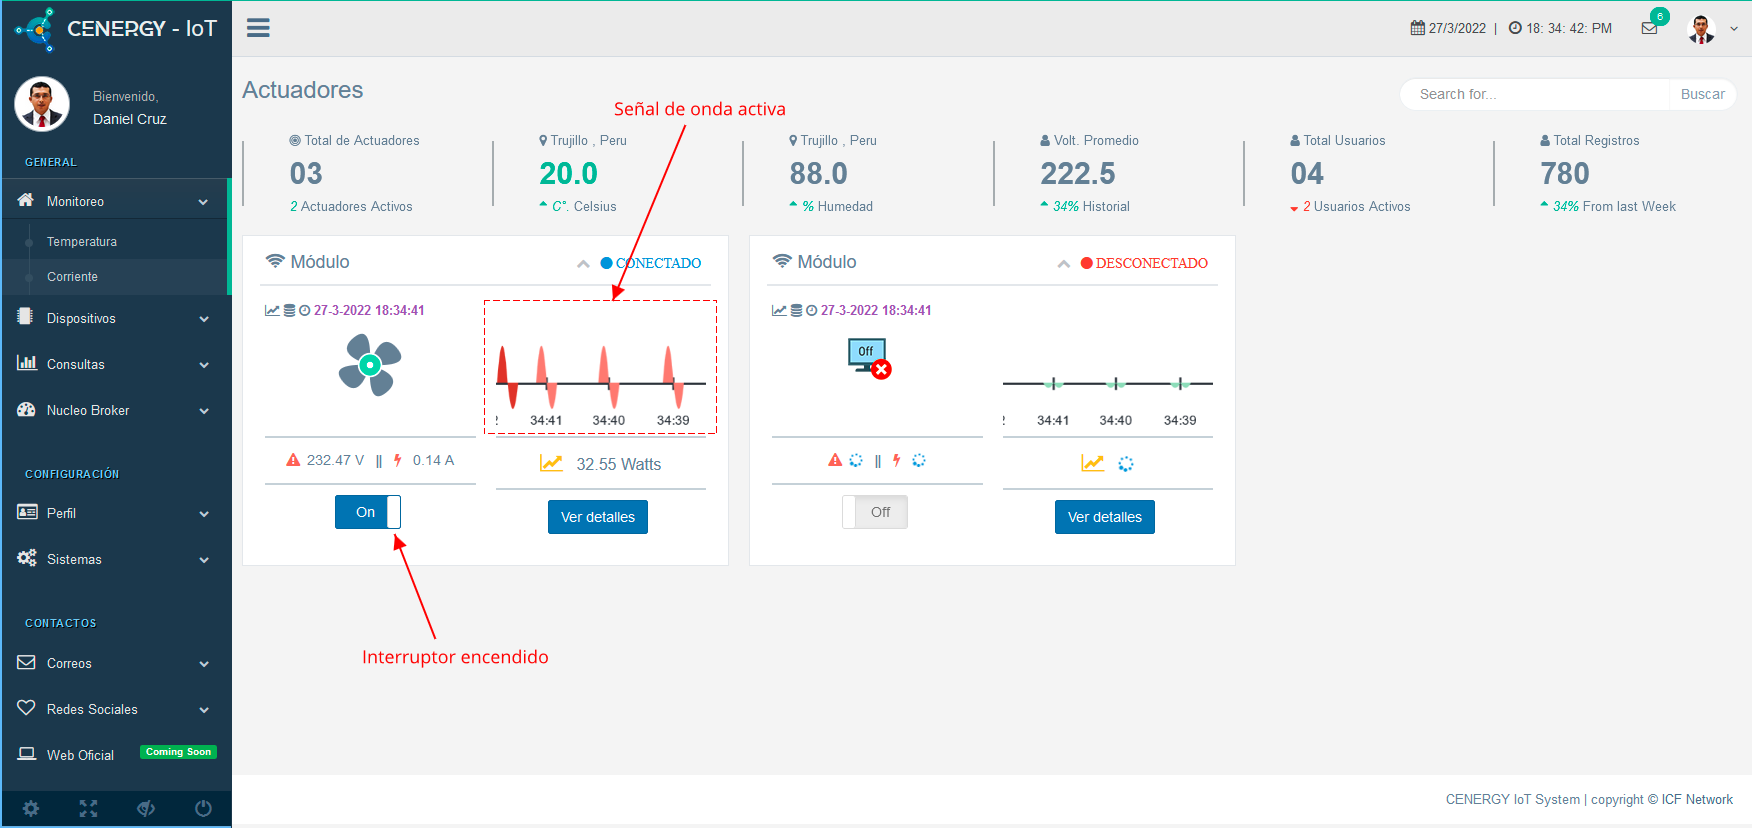
\includegraphics[width=1.7\textwidth]{./Figures/test/consumo/actuador1.png}
\caption{Visualización del módulo con paso de corriente eléctrica.}
\label{fig:dashboard-v1}
\end{figure}
\end{landscape} %
%%%%%%%%%%%%%%%%%%%%%%%%%%%%%%%%%%%%%%%%%%%%%%%%%%%
%%%%%%%%%%%%%%%%%%%%%%%%%%%%%%%%%%%%%%%%%%%%%%%%%%%
\begin{landscape} % esto es para rotar la pagina e imagen
\begin{figure}[htpb]
\centering 
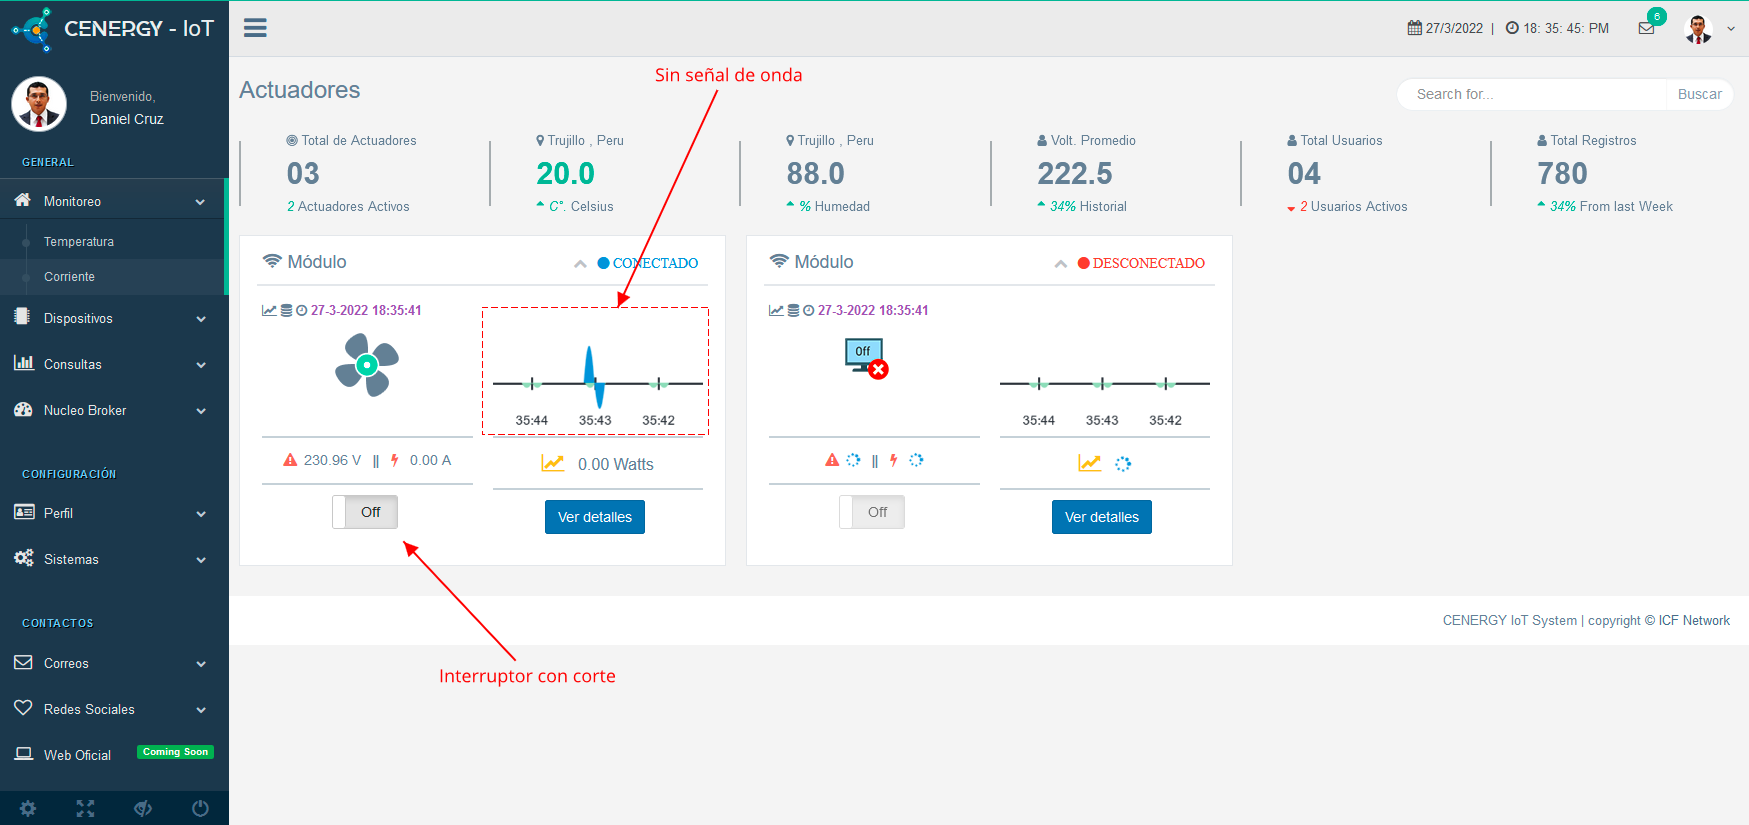
\includegraphics[width=1.7\textwidth]{./Figures/test/consumo/actuador2.png}
\caption{Visualización del módulo con bloqueo de la corriente eléctrica.}
\label{fig:dashboard-v2}
\end{figure}
\end{landscape} %
%%%%%%%%%%%%%%%%%%%%%%%%%%%%%%%%%%%%%%%%%%%%%%%%%%%
%%%%%%%%%%%%%%%%%%%%%%%%%%%%%%%%%%%%%%%%%%%%%%%%%%%
\begin{landscape} % esto es para rotar la pagina e imagen
\begin{figure}[htpb]
\centering 
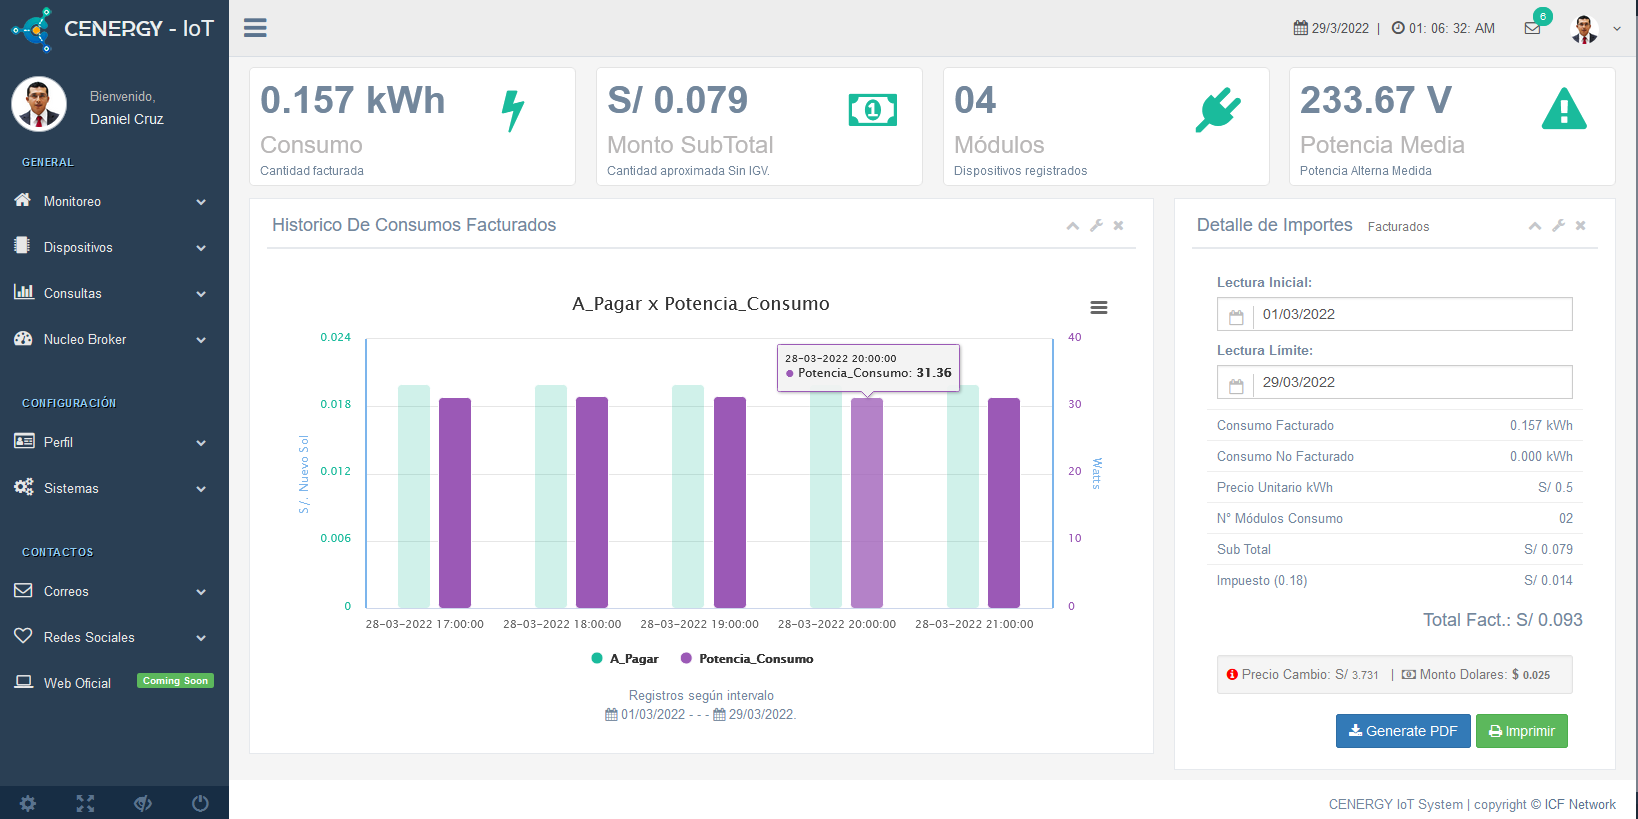
\includegraphics[width=1.7\textwidth]{./Figures/test/consumo/consumo.png}
\caption{Dashboard de facturación del software de monitoreo y control.}
\label{fig:dashboard-consumo}
\end{figure}
\end{landscape} %
%%%%%%%%%%%%%%%%%%%%%%%%%%%%%%%%%%%%%%%%%%%%%%%%%%%

Los valores obtenidos en la figura \ref{fig:dashboard-consumo} fueron contrastados con los valores ideales para el funcionamiento de 5 horas de uso, usando la ecuación \ref{eq:consumoform} tenemos la ecuación \ref{eq:ec} y \ref{eq:ec2}. 

\begin{equation}
	\label{eq:ec}
	EC = \left( 0.03 \cdot 5 \right) kW
\end{equation}

\begin{equation}
	\label{eq:ec2}
	EC = \left( 0.15 \right) kW
\end{equation}

Para obtener el costo monetario (Nuevo sol) según el consumo, se multiplica el costo por kWh con el consumo, se utilizará la última lectura de potencia entregada por el \emph{software}, que se muestra en la figura \ref{fig:dashboard-v1}, potencia igual a 32.55 W. La tabla \ref{tab:tablacostos} muestra la comparación entre los valores obtenidos, considerando el uso del ventilador por 5 horas por día, por semana (25 h) y por mes (100 h). Se consideró el costo de S/0.5 nuevos soles por cada 1 kWh.

\begin{table}[h]
	\centering
	\caption[Comparativa de consumos y costos]{Comparativa de consumos y costos.}
	\begin{tabular}{c c c c c c c}    
		\toprule
		\textbf{Pi (kW)} 	 & \textbf{Ps (kW)}  & \textbf{T (h)} &\textbf{Ci (kW)} &\textbf{Cs (kW)} &\textbf{Coi (S/)} &\textbf{Cos (S/)}\\
		\midrule
		0.03 & 0.03255 & 1 & 0.03 & 0.03255 & 0.015 & 0.016275\\		
		0.03 & 0.03255 & 5 & 0.15 & 0.16275 & 0.075 & 0.081375 \\
		0.03 & 0.03255 & 25 & 0.75 & 0.81375 & 0.375 & 0.406875\\		
		0.03 & 0.03255 & 100 & 3 & 3.255 & 1.5 & 1.6275\\		
		
		\bottomrule
		\hline
	\end{tabular}
	\label{tab:tablacostos}
\end{table}

\vspace{0.1cm}
Significado de columnas:
\begin{itemize}
\item Pi: potencia ideal (según descripción técnica del ventilador) 
\item Ps: potencia entregada por el \emph{software} de monitoreo y control
\item T: tiempo
\item Ci: consumo ideal o esperado
\item Cs: consumo entregado por el \emph{software} de monitoreo y control
\item Coi: costo ideal o esperado
\item Cos: costo calculado por el \emph{software} de monitoreo y control
\end{itemize}

\vspace{0.1cm}
De la columna Coi (valor esperado) y Cos (valor obtenido) es posible observar que los valores entregados por el \emph{software} son muy cercanos al esperado. Para obtener los errores relativos (Er) y errores absolutos (Ea) se utilizarán las ecuaciones  \ref{eq:ea} y \ref{eq:er} . La tabla \ref{tab:tablaerror} muestra los resultados de los errores obtenidos del muestreo.


%\begin{equation}
%	\label{eq:vp}
%	\overline{X} = \frac1n \cdot \sum_{i=0}^n X_i  
%\end{equation}

\begin{equation}
	\label{eq:ea}
	E_a = \left| V_r - V_a \right|
\end{equation}

\begin{equation}
	\label{eq:er}
	E_r = \left( \frac{E_a}{V_r} \right)
\end{equation}

\vspace{1.0cm}
Siendo las variables:
\begin{itemize}
\item Ea: error absoluto 
\item Er: error relativo
\item Vr: valor real o esperado
\item Va: valor aproximado o medido
\end{itemize}

\vspace{0.5cm}
\begin{table}[h]
	\centering
	\caption[Error absoluto y relativo]{Error absoluto y relativo.}
	\begin{tabular}{c c c c c}    
		\toprule
		\textbf{T (h)} & \textbf{Coi (Vr)} &\textbf{Cos (Va)} &\textbf{Ea} &\textbf{Er}\\
		\midrule
		1 & 0.015 & 0.016275 & 0.001275 & 0.085 \\		
		5 & 0.075 & 0.081375 & 0.006375 & 0.085 \\
		25 & 0.375 & 0.406875 & 0.031875 & 0.085\\		
		100 & 1.5 & 1.6275 & 0.1 & 0.067\\		
		
		\bottomrule
		\hline
	\end{tabular}
	\label{tab:tablaerror}
\end{table}

\section{Pruebas del funcionamiento del módulo replicador}

Este módulo esta compuesto con un conjunto de procesos internos que se ejecutan de forma continua dentro del sistema operativo y mostrará resultados de su salida por la terminal según su comportamiento . Resaltar que este prototipo tiene fines comerciales por tal motivo se ocultó la información sensible que usa el software para su funcionamiento.

El proceso de envío de valores a la nube esta dividido en dos subprocesos, la primera es el envío de registros mediante API remota para replicar los registros que se envían a la base de datos y la segunda el envío de valores al broker remoto. La figura \ref{fig:envia1} muestra la salida durante el llamado a la API y la figura \ref{fig:envia2} muestra la salida durante el envío al broker remoto.

\begin{figure}[htpb]
\centering 
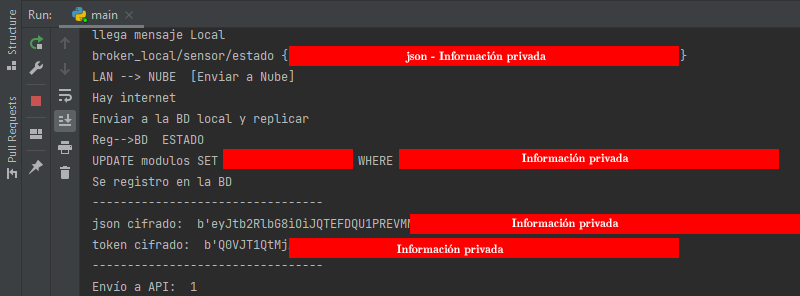
\includegraphics[width=1.0\textwidth]{./Figures/test/replicador/enviaAPI.png}
\caption{Salida de replicación a la nube usando la API.}
\label{fig:envia1}
\end{figure}

\begin{figure}[htpb]
\centering 
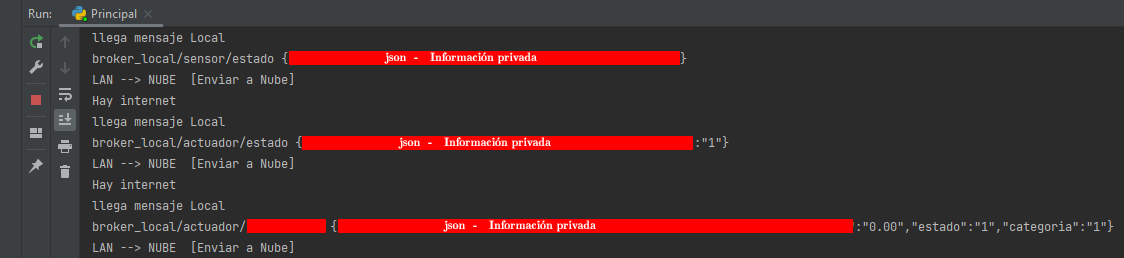
\includegraphics[width=1.0\textwidth]{./Figures/test/replicador/enviabroker.png}
\caption{Salida de replicación al broker remoto.}
\label{fig:envia2}
\end{figure}

Se mencionó en los capítulos anteriores que el replicador esta constantemente verificando si existen registros que no han sido replicados a la nube, de ser así automáticamente llamará a la API del sistema remoto para replicar los registros marcados como sin replicar. La figura \ref{fig:r1} muestra la salida el proceso sin registros por replicar y la figura \ref{fig:r2} muestra la salida al replicar usando la API. 

\begin{figure}[htpb]
\centering 
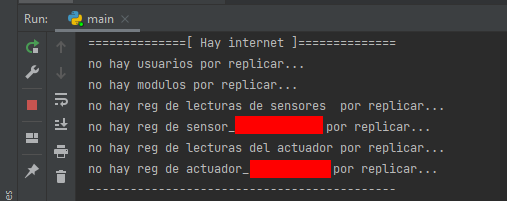
\includegraphics[width=0.8\textwidth]{./Figures/test/replicador/sinReplicar1.png}
\caption{Salida del proceso cuando no existen registros pendientes por replicar.}
\label{fig:r1}
\end{figure}

\begin{figure}[htpb]
\centering 
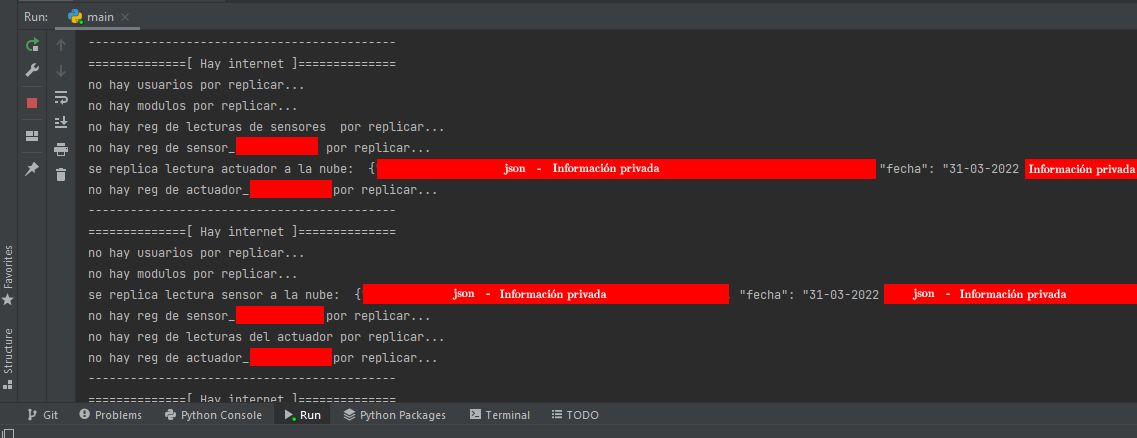
\includegraphics[width=1.0\textwidth]{./Figures/test/replicador/sinReplicar2.png}
\caption{Salida del proceso de replicación a la nube de registros marcados como pendientes.}
\label{fig:r2}
\end{figure}


\section{Pruebas del funcionamiento del sistema sin Internet}

El módulo replicador contiene un subproceso que se ejecuta de forma continua y verifica el estado del servicio de Internet. La salida del proceso se muestra en la figura \ref{fig:inter1}. 

Al estar sin Internet en la red, el sistema detecta dicho corte y muestra un mensaje en la parte superior del \emph{software} de monitoreo y control. La figura \ref{fig:inter2} y la figura \ref{fig:inter3} muestran la alerta.

%%%%%%%%%%%%%%%%%%%%%%%%%%%%%%%%%%
\begin{figure}[htpb]
\centering 
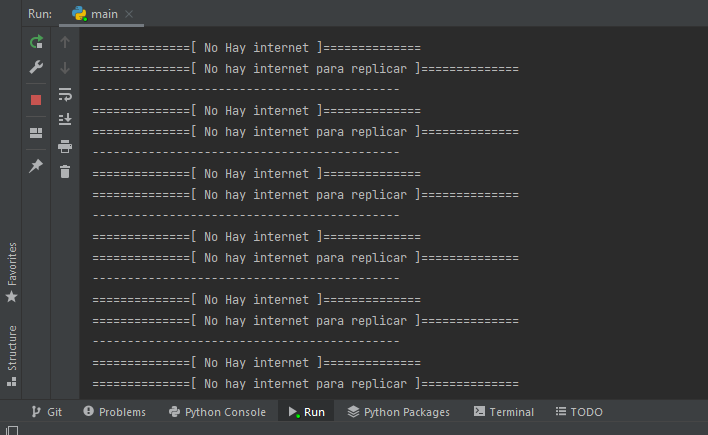
\includegraphics[width=0.6\textwidth]{./Figures/test/replicador/desconexion3.png}
\caption{Salida del proceso al detectar corte de Internet.}
\label{fig:inter1}
\end{figure}
\vspace{0.25cm}
%%%%%%%%%%%%%%%%%%%%%%%%%%%%%%
\begin{figure}[htpb]
\centering 
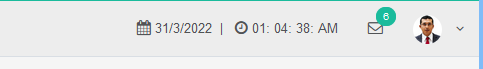
\includegraphics[width=0.7\textwidth]{./Figures/test/replicador/desconexion1.png}
\caption{Estado del software con Internet activo.}
\label{fig:inter2}
\end{figure}
%%%%%%%%%%%%%%%%%%%%%%%%%%%%%%%%%%%%%%
\begin{figure}[htpb]
\centering 

\includegraphics[width=0.7\textwidth]{./Figures/test/replicador/desconexion2.png}
\caption{Estado del software sin Internet.}
\label{fig:inter3}
\end{figure}


\section{Pruebas del sistema desde acceso remoto}

Para visualizar la comunicación entre el \emph{software} réplica - remoto y el módulo principal local se muestra el grafo del funcionamiento del sistema de monitoreo y control. El software nos permite visualizar en tiempo real el comportamiento y el envió de mensajes entre canales como se muestra en la figura \ref{fig:graforemoto}. Los puntos de colores en la figura significan:

\begin{itemize}
\item Punto negro: mensaje enviado.
\item Punto rojo: cliente remoto conectado al sistema IoT.
\item Punto azul: cliente conectado al broker remoto en modo escucha.
\item Punto naranja: mensaje de un cliente remoto conectado temporalmente para enviar sincronizacion de estados desde el remoto al modulo principal local. 
\end{itemize}

%%%%%%%%%%%%%%%%%%%%%%%%%%%%%%%%%%%%%%%%%%%%%%%%%%%
\begin{landscape} % esto es para rotar la pagina e imagen
\begin{figure}[htpb]
\centering 
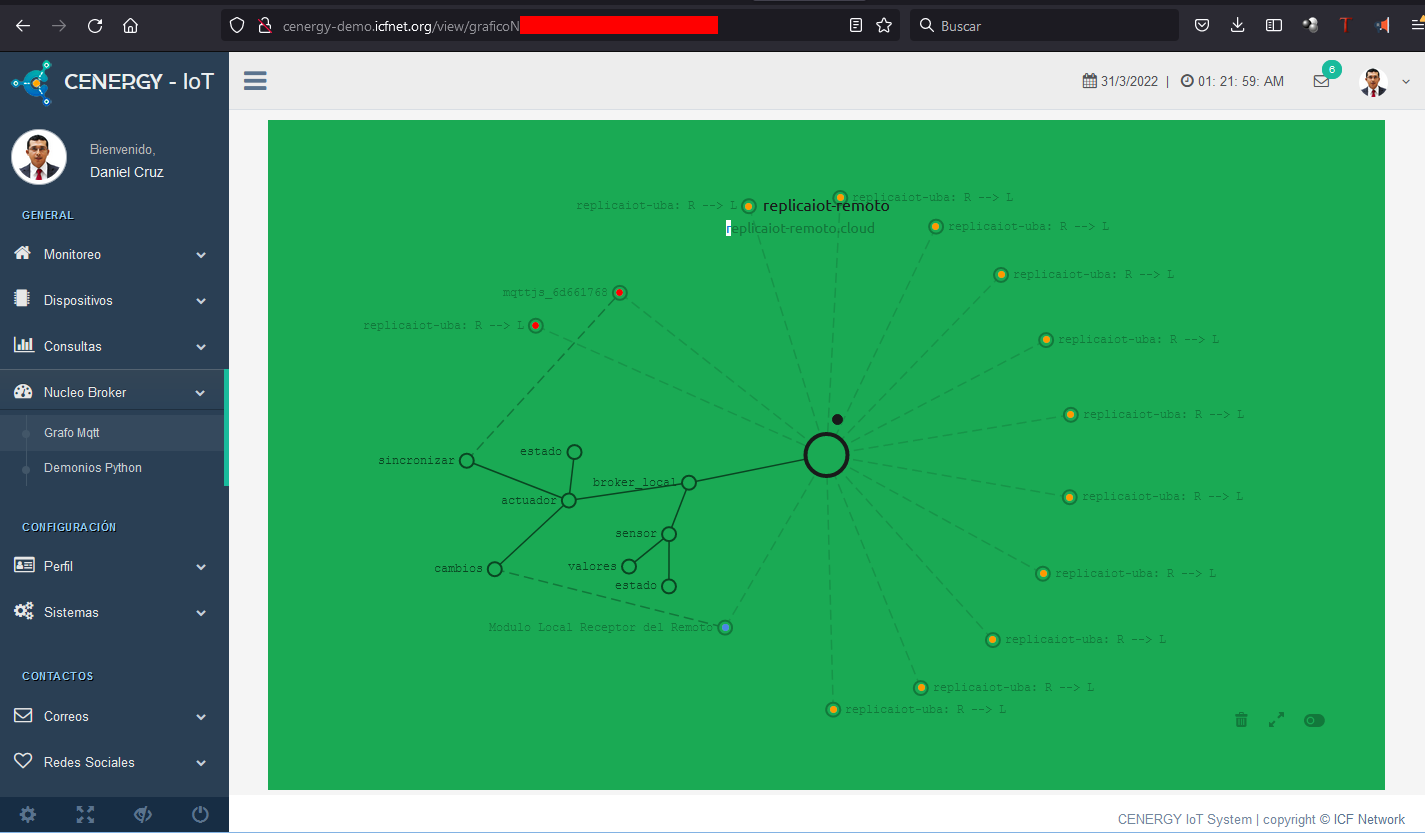
\includegraphics[width=1.6\textwidth]{./Figures/test/replicador/remoto.png}
\caption{Grafo de comunicación MQTT funcionando desde el sistema réplica en la nube.}
\label{fig:graforemoto}
\end{figure}
\end{landscape} 
%%%%%%%%%%%%%%%%%%%%%%%%%%%%%%%%%%%%%%%%%%%%%%%%%%%

\section{Comparativa del resultado con soluciones similares}

Una vez expuestos los resultados obtenidos para cada módulo, se presenta a continuación el análisis de los resultados comparativos entre los tres tipos de soluciones descritos en el capítulo 1. La tabla \ref{tab:tabla-resultado} permite determinar las diferencias significativas con el uso y el tipo de servidor contra cada una de las diferentes soluciones.

\begin{table}[h]
	\centering
	\caption[Comparativa de soluciones entre acceso y servidor]{Comparativa acceso y tipo de servidor.}
	\begin{tabular}{l c c c c }    
		\toprule
		\textbf{Producto} & \textbf{Acceso}  & \textbf{Uso} & \textbf{S. local}   & \textbf{S. remoto} \\
		\midrule
		Energy Manager & Local y remoto 	& navegador & no & sí  \\		
		Iammeter	 & local y remoto	& navegador y app. & no & sí  \\
		Bee2energy	 & local y remoto	& navegador & no & sí  \\
		\rowcolor[HTML]{ebedef}Cenergy IoT System & local y remoto& navegador & sí & sí \\
		\bottomrule
		\hline
	\end{tabular}
	\label{tab:tabla-resultado}
\end{table}

%%%%%%%%%%%%%%%%%%%%%%

La tabla \ref{tab:tabla-resultado2} permite determinar las diferencias respecto al uso de protocolos y el tipo de módulos que usa cada solución. 


\begin{table}[h]
	\centering
	\caption[Comparativa de soluciones entre protocolo y hardware]{Comparativa protocolo y tipos de hardware.}
	\begin{tabular}{l p{5cm} p{5cm}}    
		\toprule
		\textbf{Producto} 	 & \textbf{Protocolos}  & \textbf{M. sensores y actuadores}  \\
		\midrule
		Energy Manager & Modbus, M-Bus y TCP/IP 	& diseños propios \\		
		Iammeter	 & MQTT y TCP/IP	&diseños propios y compatibles con       dispositivos Sonoff   \\
		Bee2energy	 & múltiples protocolos IoT		& diseños propios y compatibles con otros comerciales  \\
		\rowcolor[HTML]{ebedef}Cenergy IoT	System & MQTT y TCP/IP		&diseños propios  \\
		\bottomrule
		\hline
	\end{tabular}
	\label{tab:tabla-resultado2}
\end{table}
